% Requires in the preamble:
% \usepackage{amsmath,amssymb}
% \usepackage{tikz,pgfplots}
% \pgfplotsset{compat=1.18}

\chapter{What Integrals Measure}
\label{chap:what-integrals-measure}

In Chapter \ref{chap:integral-as-accumulation}, the foundational slice was a rectangle: 
\[
\text{height}\cdot\text{width}.
\]
Moving forward, the geometry of the slice will adapt to the problem. For the area between curves, the slice is a vertical strip. For the volume of a solid, the slice is a thin cross-section. 

Geometry is only the beginning. Integrals can just as easily accumulate mass, mechanical work, fluid pressure, or probability. In every new application, the formula and units of the slice will change. But while the definition of the slice varies wildly from problem to problem, the underlying architecture of the calculus does not. Every application relies on the exact same sequence:

\[
\boxed{
\text{isolate a differential slice, approximate its contribution, and integrate to accumulate the total.}
}
\]

\section{Area between curves}
\label{sec:area-between-curves}

Area under a graph measures the region between the graph and the \(x\)-axis.  But the
\(x\)-axis is only one possible lower boundary.

Often a region lies between two curves.  Then the vertical thickness of a small strip is
not ``height above the axis.''  It is

\[
\text{top value}-\text{bottom value}.
\]

That is the first new small piece.

\subsection{Top minus bottom}
\label{subsec:top-minus-bottom}

Suppose two continuous functions \(f\) and \(g\) satisfy

\[
g(x)\ge f(x)
\]

on the interval \([a,b]\).  The region between their graphs is made of thin vertical
strips.

At a particular \(x\), the top of the strip has height \(g(x)\), and the bottom has height
\(f(x)\).  So the strip height is

\[
g(x)-f(x).
\]

If the strip has small width \(\Delta x\), then its area is approximately

\[
\bigl(g(x)-f(x)\bigr)\Delta x.
\]

Adding the strips and taking the limit gives the area.

\begin{quote}
\textbf{Area between two curves, vertical slices.}
If \(g(x)\ge f(x)\) on \([a,b]\), then the area between the graphs of \(y=g(x)\) and
\(y=f(x)\) from \(x=a\) to \(x=b\) is

\[
\boxed{
A=\int_a^b \bigl(g(x)-f(x)\bigr)\,dx.
}
\]
\end{quote}

In words:

\[
\boxed{
\text{area}=\int(\text{top}-\text{bottom})\,dx.
}
\]

The order matters.  Area is positive.  The height of a vertical strip is top minus bottom,
not bottom minus top.

\paragraph{Example: a line over a parabola.}
Find the area enclosed by

\[
y=2x
\]

and

\[
y=x^2.
\]

First find the intersection points:

\[
2x=x^2.
\]

So

\[
x^2-2x=0,
\]

and therefore

\[
x(x-2)=0.
\]

The curves meet at

\[
x=0
\qquad\text{and}\qquad
x=2.
\]

On \(0<x<2\), the line is above the parabola.  For example, at \(x=1\),

\[
2x=2
\qquad\text{and}\qquad
x^2=1.
\]

Thus

\[
\text{top}=2x,
\qquad
\text{bottom}=x^2.
\]

The area is

\[
A=\int_0^2 (2x-x^2)\,dx.
\]

Compute:

\[
A
=
\left(x^2-\frac{x^3}{3}\right)\Big|_0^2
=
\left(4-\frac83\right)-0
=
\boxed{\frac43}.
\]

\begin{figure}[h]
\centering
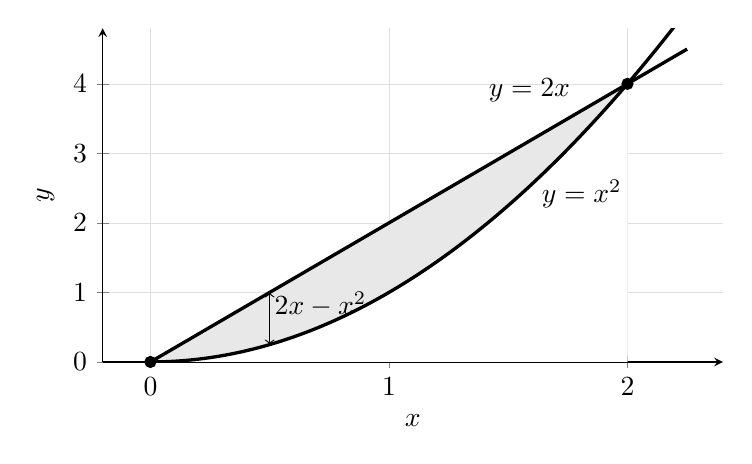
\begin{tikzpicture}
\begin{axis}[
    width=0.78\textwidth,
    height=0.48\textwidth,
    xmin=-0.2, xmax=2.4,
    ymin=0, ymax=4.8,
    axis lines=left,
    xlabel={\(x\)},
    ylabel={\(y\)},
    xtick={0,1,2},
    ytick={0,1,2,3,4},
    grid=both,
    grid style={line width=.1pt, draw=gray!25},
]
% Fill under top, then remove under bottom.
\addplot[domain=0:2, samples=100, fill=gray!18, draw=none] {2*x} \closedcycle;
\addplot[domain=0:2, samples=100, fill=white, draw=none] {x^2} \closedcycle;

% Curves
\addplot[very thick, domain=0:2.25, samples=2] {2*x};
\addplot[very thick, domain=0:2.25, samples=100] {x^2};

% Adjusted arrow matching the curves exactly at x=0.5
\draw[<->] (axis cs:0.5,0.25) -- (axis cs:0.5,1);
\node[anchor=west] at (axis cs:0.48,0.825) {\(2x-x^2\)};

\addplot[only marks, mark=*] coordinates {(0,0) (2,4)};

% Repositioned labels anchored cleanly away from the functions
\node[anchor=south east] at (axis cs:1.8, 3.6) {\(y=2x\)};
\node[anchor=north west] at (axis cs:1.6, 2.76) {\(y=x^2\)};
\end{axis}
\end{tikzpicture}
\caption{A vertical strip has height \(2x-x^2\), so the area is \(\int_0^2(2x-x^2)\,dx\).}
\label{fig:area-line-parabola}
\end{figure}
The integral did not measure area under one graph.  It measured accumulated strip
heights between two graphs.

\subsection{Why we cannot skip the picture}
\label{subsec:why-area-picture-matters}

The formula

\[
\int_a^b (\text{top}-\text{bottom})\,dx
\]

requires knowing which graph is on top.  That may change.

Consider the curves

\[
y=x
\]

and

\[
y=x^3.
\]

They intersect when

\[
x=x^3.
\]

So

\[
x^3-x=0,
\]

or

\[
x(x-1)(x+1)=0.
\]

The intersection points occur at

\[
x=-1,\quad x=0,\quad x=1.
\]

On the interval \([-1,0]\), the cubic is above the line.  For example, at \(x=-1/2\),

\[
x^3=-\frac18
\qquad\text{and}\qquad
x=-\frac12,
\]

so

\[
x^3>x.
\]

On the interval \([0,1]\), the line is above the cubic.  For example, at \(x=1/2\),

\[
x=\frac12
\qquad\text{and}\qquad
x^3=\frac18,
\]

so

\[
x>x^3.
\]

Therefore the area is

\[
A
=
\int_{-1}^0 (x^3-x)\,dx
+
\int_0^1 (x-x^3)\,dx.
\]

Compute the two equal parts:

\[
\int_0^1 (x-x^3)\,dx
=
\left(\frac{x^2}{2}-\frac{x^4}{4}\right)\Big|_0^1
=
\frac12-\frac14
=
\frac14.
\]

Thus

\[
A=\frac14+\frac14=\boxed{\frac12}.
\]

If we had written

\[
\int_{-1}^1 (x-x^3)\,dx,
\]

we would have gotten

\[
0,
\]

because the positive and negative signed areas cancel.  That is not the area of the
region.

\begin{quote}
\textbf{Warning.}
Area between curves is not found by blindly integrating one function minus the other.
The integrand must be

\[
\text{top}-\text{bottom}.
\]

If the top curve changes, split the integral.
\end{quote}

This is the same lesson we learned with signed area.  A definite integral may cancel
positive and negative contributions.  Ordinary area does not cancel.

\subsection{Right minus left}
\label{subsec:right-minus-left}

Vertical slices are not always the easiest choice.  Sometimes a horizontal strip has a
simpler length.

For a horizontal strip, the small thickness is \(dy\).  Its length is

\[
\text{right value}-\text{left value}.
\]

So the small area is

\[
(\text{right}-\text{left})\,dy.
\]

\begin{quote}
\textbf{Area between curves, horizontal slices.}
If \(r(y)\ge \ell(y)\) on \([c,d]\), then the area between the curves
\(x=r(y)\) and \(x=\ell(y)\) is

\[
\boxed{
A=\int_c^d \bigl(r(y)-\ell(y)\bigr)\,dy.
}
\]
\end{quote}

In words:

\[
\boxed{
\text{area}=\int(\text{right}-\text{left})\,dy.
}
\]

\paragraph{Example: two sideways parabolas.}
Find the area enclosed by

\[
x=y^2
\]

and

\[
x=2-y^2.
\]

The curves meet when

\[
y^2=2-y^2.
\]

Thus

\[
2y^2=2,
\]

so

\[
y^2=1,
\qquad
y=\pm1.
\]

For \(-1\le y\le1\), the right boundary is

\[
x=2-y^2,
\]

and the left boundary is

\[
x=y^2.
\]

Therefore the area is

\[
A=\int_{-1}^1 \bigl((2-y^2)-y^2\bigr)\,dy.
\]

So

\[
A=\int_{-1}^1 (2-2y^2)\,dy.
\]

Compute:

\[
A
=
\left(2y-\frac{2y^3}{3}\right)\Big|_{-1}^{1}.
\]

At \(y=1\), this gives

\[
2-\frac23=\frac43.
\]

At \(y=-1\), it gives

\[
-2+\frac23=-\frac43.
\]

So

\[
A=\frac43-\left(-\frac43\right)=\boxed{\frac83}.
\]

\begin{figure}[h]
\centering
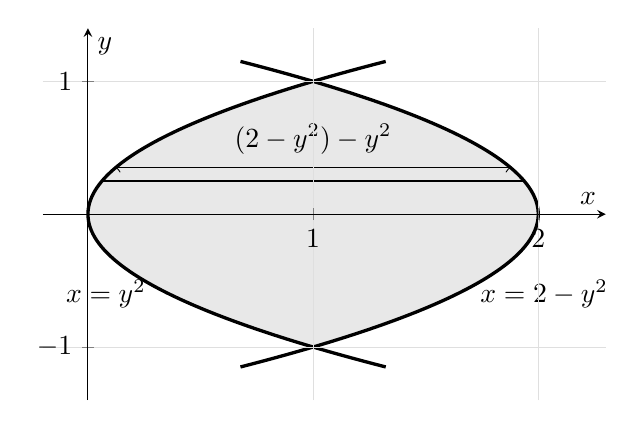
\begin{tikzpicture}
\begin{axis}[
    width=0.72\textwidth,
    height=0.52\textwidth,
    xmin=-0.2, xmax=2.3,
    ymin=-1.4, ymax=1.4,
    axis lines=middle,
    axis on top,
    xlabel={\(x\)},
    ylabel={\(y\)},
    xtick={0,1,2},
    ytick={-1,0,1},
    grid=both,
    grid style={line width=.1pt, draw=gray!25},
]
% Fill region by horizontal-looking polygon coordinates.
\addplot[fill=gray!18, draw=none] coordinates {
    (1, -1) (0.81, -0.9) (0.64, -0.8) (0.49, -0.7) (0.36, -0.6) (0.25, -0.5)
    (0.16, -0.4) (0.09, -0.3) (0.04, -0.2) (0.01, -0.1) (0, 0) (0.01, 0.1)
    (0.04, 0.2) (0.09, 0.3) (0.16, 0.4) (0.25, 0.5) (0.36, 0.6) (0.49, 0.7)
    (0.64, 0.8) (0.81, 0.9) (1, 1) (1, 1) (1.19, 0.9) (1.36, 0.8) (1.51, 0.7)
    (1.64, 0.6) (1.75, 0.5) (1.84, 0.4) (1.91, 0.3) (1.96, 0.2) (1.99, 0.1)
    (2, 0) (1.99, -0.1) (1.96, -0.2) (1.91, -0.3) (1.84, -0.4) (1.75, -0.5)
    (1.64, -0.6) (1.51, -0.7) (1.36, -0.8) (1.19, -0.9) (1, -1)
};

\addplot[very thick, domain=-1.15:1.15, samples=100] ({x^2},{x});
\addplot[very thick, domain=-1.15:1.15, samples=100] ({2-x^2},{x});

% Typical horizontal strip lowered to y=0.25
% x_left = (0.25)^2 = 0.0625, x_right = 2 - (0.25)^2 = 1.9375
\draw[thick] (axis cs:0.0625,0.25) -- (axis cs:1.9375,0.25);

% Dimension arrow at y=0.35, correctly calculated to touch the curves
% x_left = (0.35)^2 = 0.1225, x_right = 2 - (0.35)^2 = 1.8775
\draw[<->] (axis cs:0.1225,0.35) -- (axis cs:1.8775,0.35);

% Label anchored slightly above the arrow
\node[anchor=south] at (axis cs:1.0,0.38) {\((2-y^2)-y^2\)};

% Curve labels anchored closely to the lower branches
\node[anchor=east] at (axis cs:0.3,-0.6) {\(x=y^2\)};
\node[anchor=west] at (axis cs:1.7,-0.6) {\(x=2-y^2\)};

\end{axis}
\end{tikzpicture}
\caption{A horizontal strip has length \((2-y^2)-y^2\), so we integrate with respect to \(y\).}
\label{fig:right-minus-left-sideways-parabolas}
\end{figure}

A vertical slice would have forced us to split the region into several pieces.  A horizontal
slice sees the whole region at once.

\subsection{Splitting at intersections}
\label{subsec:splitting-at-intersections}

Intersections are not just endpoints.  They are places where the description of the
region may change.

Here is a safe procedure.

\begin{quote}
\textbf{Setting up an area between curves.}

\begin{enumerate}
\item Draw or imagine the region.
\item Find the intersection points.
\item Decide whether vertical or horizontal slices are simpler.
\item Write the height or length of a typical slice.
\item Split the integral wherever the top/bottom or right/left description changes.
\end{enumerate}
\end{quote}

The picture is not decoration.  It tells which subtraction is legal.

\paragraph{Example: one region, two vertical descriptions.}
Find the area of the region bounded by

\[
y=x^2
\]

and

\[
y=2-x.
\]

First find intersections:

\[
x^2=2-x.
\]

So

\[
x^2+x-2=0,
\]

and therefore

\[
(x+2)(x-1)=0.
\]

The curves meet at

\[
x=-2
\qquad\text{and}\qquad
x=1.
\]

On the interval \([-2,1]\), test \(x=0\):

\[
x^2=0,
\qquad
2-x=2.
\]

Thus the line is on top and the parabola is on the bottom.  The area is

\[
A=\int_{-2}^1 \bigl((2-x)-x^2\bigr)\,dx.
\]

Compute:

\[
A
=
\int_{-2}^1 (2-x-x^2)\,dx
=
\left(2x-\frac{x^2}{2}-\frac{x^3}{3}\right)\Big|_{-2}^{1}.
\]

At \(x=1\),

\[
2-\frac12-\frac13=\frac76.
\]

At \(x=-2\),

\[
-4-2+\frac83=-\frac{10}{3}.
\]

So

\[
A=\frac76-\left(-\frac{10}{3}\right)
=
\frac76+\frac{20}{6}
=
\boxed{\frac{27}{6}}
=
\boxed{\frac92}.
\]

In this example the top curve did not change.  But we still found the intersections first
because they gave the interval of integration.

\subsection{Area from data and graphs}
\label{subsec:area-from-data-and-graphs}

A formula is not always available.  If a graph or table gives the vertical distance between
two boundaries, the same idea still works.

Suppose a surveyor measures the distance between two shorelines at equally spaced
values of \(x\).  The distances are:

\begin{center}
\begin{tabular}{c|ccccc}
\(x\) & \(0\) & \(1\) & \(2\) & \(3\) & \(4\) \\ \hline
vertical distance & \(0\) & \(3\) & \(4\) & \(2\) & \(0\)
\end{tabular}
\end{center}

The spacing is

\[
\Delta x=1.
\]

Using the trapezoid rule, the area is approximately

\[
1\left(\frac12(0)+3+4+2+\frac12(0)\right)=9.
\]

So the area is approximately

\[
9
\]

square units.

The same calculation can be written as an approximate integral:

\[
A=\int_0^4 (\text{top}-\text{bottom})\,dx
\approx 9.
\]

The data gave the height difference directly.  If the data instead gave separate top and
bottom values, we would subtract first and then estimate the integral.

\begin{quote}
\textbf{Data version.}
When the boundary is measured rather than given by formulas, the integral is still built
from the same small piece:

\[
(\text{measured strip height})(\text{strip width}).
\]

A table changes how we estimate the integral, not what the integral means.
\end{quote}

Area between curves is still area.  We have only replaced a rectangle under one curve
by a strip between two curves.  The next step changes dimension.  A strip becomes a
slice.

\section{Volumes by slicing}
\label{sec:volumes-by-slicing}

Area is two-dimensional accumulation.  Volume is three-dimensional accumulation.

The idea is familiar from a loaf of bread.  If we know the area of each slice and the
thickness of the slices, then the volume is approximately

\[
\text{slice area}\cdot\text{slice thickness}
\]

added over all slices.

As the slices become thinner, the approximation becomes an integral.

\subsection{Cross-sectional area as a function}
\label{subsec:cross-sectional-area-function}

Suppose a solid stretches from \(x=a\) to \(x=b\).  At each \(x\), cut the solid by a plane
perpendicular to the \(x\)-axis.  Let

\[
A(x)
\]

be the area of that cross section.

A thin slice near \(x\) with thickness \(\Delta x\) has volume approximately

\[
A(x)\Delta x.
\]

Add the slices:

\[
A(x_1)\Delta x+A(x_2)\Delta x+\cdots+A(x_n)\Delta x.
\]

Taking the limit gives the volume.

\begin{quote}
\textbf{Volume by slicing.}
If a solid lies between \(x=a\) and \(x=b\), and if the cross-sectional area perpendicular
to the \(x\)-axis is \(A(x)\), then

\[
\boxed{
V=\int_a^b A(x)\,dx.
}
\]
\end{quote}

The unit check is useful.  If \(A(x)\) is measured in square centimeters and \(dx\) is
measured in centimeters, then

\[
A(x)\,dx
\]

has units

\[
\text{cm}^2\cdot\text{cm}=\text{cm}^3.
\]

That is volume.

\begin{figure}[h]
\centering
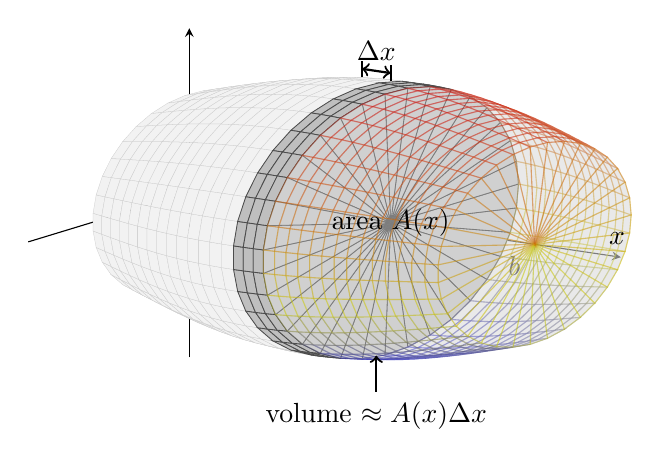
\begin{tikzpicture}
\begin{axis}[
    view={35}{20},
    width=0.95\textwidth,
    height=0.65\textwidth,
    grid=none,
    axis lines=center,
    xlabel={\(x\)},
    ylabel={},
    zlabel={},
    xtick={0, 3, 3.5, 6},
    xticklabels={\(a\), \(x\), \(x+\Delta x\), \(b\)},
    ytick=\empty,
    ztick=\empty,
    xmin=-0.5, xmax=7.5,
    ymin=-2.5, ymax=2.5,
    zmin=-2.5, zmax=2.5,
    z buffer=sort
]

% 1. Back portion of the solid (x from 0 to 3)
\addplot3[
    surf,
    domain=0:3,
    y domain=0:360,
    samples=15,
    samples y=36,
    fill=gray!10,
    faceted color=gray!40,
    line width=0.1pt
] (
    {x},
    {(1.5 + 0.5*sin(x*30)) * cos(y)},
    {(1.5 + 0.5*sin(x*30)) * sin(y)}
);

% 2. Solid cap at x=3 (Back wall of the slice)
\addplot3[
    surf,
    domain=0:1,
    y domain=0:360,
    samples=2,
    samples y=36,
    fill=gray!30,
    faceted color=gray!50,
    line width=0.1pt
] (
    {3},
    {2.0 * x * cos(y)},
    {2.0 * x * sin(y)}
);

% 3. The highlighted differential slice crust (x from 3 to 3.5)
\addplot3[
    surf,
    domain=3:3.5,
    y domain=0:360,
    samples=4,
    samples y=36,
    fill=gray!50,
    faceted color=black!70,
    line width=0.3pt
] (
    {x},
    {(1.5 + 0.5*sin(x*30)) * cos(y)},
    {(1.5 + 0.5*sin(x*30)) * sin(y)}
);

% 4. Solid cap at x=3.5 (Front face of the slice)
\addplot3[
    surf,
    domain=0:1,
    y domain=0:360,
    samples=2,
    samples y=36,
    fill=gray!40,
    faceted color=black!70,
    line width=0.3pt
] (
    {3.5},
    {1.9829 * x * cos(y)}, 
    {1.9829 * x * sin(y)}
);

% 5. Front portion of the solid (x from 3.5 to 6) - TRANSPARENT
\addplot3[
    surf,
    domain=3.5:6,
    y domain=0:360,
    samples=15,
    samples y=36,
    fill=gray!30,
    draw=none, % No grid
    opacity=0.35 % See-through
] (
    {x},
    {(1.5 + 0.5*sin(x*30)) * cos(y)},
    {(1.5 + 0.5*sin(x*30)) * sin(y)}
);

% 6. End cap at x=6 - TRANSPARENT
\addplot3[
    surf,
    domain=0:1,
    y domain=0:360,
    samples=2,
    samples y=36,
    fill=gray!30,
    draw=none,
    opacity=0.35
] (
    {6},
    {1.5 * x * cos(y)},
    {1.5 * x * sin(y)}
);

% --- Annotations ---

% Delta x dimension bracket at the top
\draw[thick] (axis cs:3.0, 0, 2.15) -- (axis cs:3.0, 0, 2.4);
\draw[thick] (axis cs:3.5, 0, 2.15) -- (axis cs:3.5, 0, 2.4);
\draw[thick, <->] (axis cs:3.0, 0, 2.275) -- (axis cs:3.5, 0, 2.275) node[midway, above] {\(\Delta x\)};

% Area label directly on the face of the slice
\node at (axis cs:3.5, 0, 0) {area \(A(x)\)};

% Volume label pointing to the bottom of the slice
\node[anchor=north] at (axis cs:3.25, 0, -2.6) {volume \(\approx A(x)\Delta x\)};
\draw[thick, <-] (axis cs:3.25, 0, -2.05) -- (axis cs:3.25, 0, -2.6);

\end{axis}
\end{tikzpicture}
\caption{Volume by slicing: a differential slice of thickness \(\Delta x\) has volume approximately \(A(x)\Delta x\).}
\label{fig:volume-by-slicing-loaf}
\end{figure}

This formula is simple, but it hides the real work.  The hard part is finding \(A(x)\).

\paragraph{Example: a cone from its cross sections.}
A right circular cone has height \(h\) and base radius \(R\).  Put the vertex at \(x=0\)
and the base at \(x=h\).  At position \(x\), the cross section perpendicular to the
\(x\)-axis is a disk.

The radius grows linearly from \(0\) to \(R\).  By similar triangles,

\[
r(x)=\frac{R}{h}x.
\]

So the cross-sectional area is

\[
A(x)=\pi r(x)^2
=
\pi\left(\frac{R}{h}x\right)^2
=
\frac{\pi R^2}{h^2}x^2.
\]

The volume is

\[
V=\int_0^h A(x)\,dx
=
\int_0^h \frac{\pi R^2}{h^2}x^2\,dx.
\]

Compute:

\[
V
=
\frac{\pi R^2}{h^2}
\left(\frac{x^3}{3}\right)\Big|_0^h
=
\frac{\pi R^2}{h^2}\cdot \frac{h^3}{3}
=
\boxed{\frac13\pi R^2h}.
\]

This is the familiar cone formula.  The integral explains the factor \(1/3\): the cross
sections grow like \(x^2\), and

\[
\int_0^h x^2\,dx=\frac{h^3}{3}.
\]

\subsection{Solids of revolution: disks and washers}
\label{subsec:solids-of-revolution-disks-washers}

A common way to make a solid is to rotate a plane region around an axis.  The resulting
solid is called a \emph{solid of revolution}.

If a vertical slice rotates around the \(x\)-axis, it sweeps out a disk or a washer.

\paragraph{Disk slices.}
Suppose \(f(x)\ge0\) on \([a,b]\).  Rotate the region under

\[
y=f(x)
\]

above the \(x\)-axis around the \(x\)-axis.

At position \(x\), the cross section perpendicular to the \(x\)-axis is a disk with radius

\[
f(x).
\]

So

\[
A(x)=\pi f(x)^2.
\]

Therefore

\[
\boxed{
V=\pi\int_a^b f(x)^2\,dx.
}
\]

\paragraph{Example: rotating \(y=\sqrt{x}\).}
Rotate the region under

\[
y=\sqrt{x}
\]

from \(x=0\) to \(x=4\) around the \(x\)-axis.

A cross section at \(x\) is a disk with radius

\[
\sqrt{x}.
\]

So

\[
A(x)=\pi(\sqrt{x})^2=\pi x.
\]

Thus

\[
V=\int_0^4 \pi x\,dx
=
\pi\left(\frac{x^2}{2}\right)\Big|_0^4
=
\boxed{8\pi}.
\]

\begin{figure}[h]
\centering
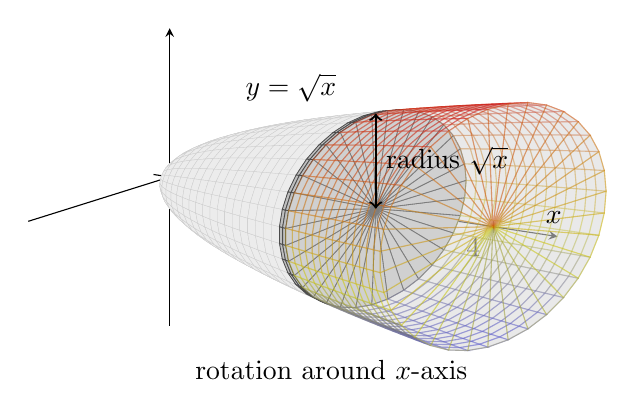
\begin{tikzpicture}
\begin{axis}[
    view={35}{20},
    width=0.85\textwidth,
    height=0.6\textwidth,
    grid=none,
    axis lines=center,
    xlabel={\(x\)},
    ylabel={},
    zlabel={},
    xtick={0, 2.5, 4},
    xticklabels={\(0\), \(x\), \(4\)},
    ytick=\empty,
    ztick=\empty,
    xmin=-0.2, xmax=4.8,
    ymin=-2.5, ymax=2.5,
    zmin=-2.5, zmax=2.5,
    z buffer=sort
]

% 1. Back portion of the solid (x from 0 to 2.45)
\addplot3[
    surf,
    domain=0:2.45,
    y domain=0:360,
    samples=20,
    samples y=36,
    fill=gray!15,
    faceted color=gray!40,
    line width=0.1pt
] (
    {x},
    {sqrt(x) * cos(y)},
    {sqrt(x) * sin(y)}
);

% 2. Back cap of the disk slice (x=2.45)
\addplot3[
    surf,
    domain=0:1,
    y domain=0:360,
    samples=2,
    samples y=36,
    fill=gray!30,
    faceted color=gray!50,
    line width=0.1pt
] (
    {2.45},
    {sqrt(2.45) * x * cos(y)},
    {sqrt(2.45) * x * sin(y)}
);

% 3. The highlighted differential disk crust (x from 2.45 to 2.55)
\addplot3[
    surf,
    domain=2.45:2.55,
    y domain=0:360,
    samples=3,
    samples y=36,
    fill=gray!50,
    faceted color=black!70,
    line width=0.3pt
] (
    {x},
    {sqrt(x) * cos(y)},
    {sqrt(x) * sin(y)}
);

% 4. Front face of the disk slice (x=2.55)
\addplot3[
    surf,
    domain=0:1,
    y domain=0:360,
    samples=2,
    samples y=36,
    fill=gray!40,
    faceted color=black!70,
    line width=0.3pt
] (
    {2.55},
    {sqrt(2.55) * x * cos(y)},
    {sqrt(2.55) * x * sin(y)}
);

% 5. Front portion of the solid (x from 2.55 to 4) - TRANSPARENT
\addplot3[
    surf,
    domain=2.55:4,
    y domain=0:360,
    samples=15,
    samples y=36,
    fill=gray!30,
    draw=none, % No grid
    opacity=0.35 % See-through
] (
    {x},
    {sqrt(x) * cos(y)},
    {sqrt(x) * sin(y)}
);

% 6. End cap at x=4 - TRANSPARENT
\addplot3[
    surf,
    domain=0:1,
    y domain=0:360,
    samples=2,
    samples y=36,
    fill=gray!30,
    draw=none,
    opacity=0.35
] (
    {4},
    {2 * x * cos(y)}, % sqrt(4) = 2
    {2 * x * sin(y)}
);

% --- Annotations ---

% Radius line directly on the front face of the disk slice
\draw[thick, <->] (axis cs:2.55, 0, 0) -- (axis cs:2.55, 0, 1.5968) node[midway, right] {radius \(\sqrt{x}\)};

% Curve label floating along the upper edge
\node[anchor=south] at (axis cs:1.5, 0, 1.4) {\(y=\sqrt{x}\)};

% Rotation label below the solid
\node[anchor=north] at (axis cs:2.0, 0, -2.5) {rotation around \(x\)-axis};

\end{axis}
\end{tikzpicture}
\caption{Rotating the region under \(y=\sqrt{x}\) around the \(x\)-axis gives disk slices.}
\label{fig:disk-method-sqrtx}
\end{figure}

\paragraph{Washer slices.}
If a region has a hole after rotation, the cross sections are washers.

Suppose \(R(x)\ge r(x)\ge0\).  Rotate the region between

\[
y=R(x)
\]

and

\[
y=r(x)
\]

around the \(x\)-axis.  The outer radius is \(R(x)\).  The inner radius is \(r(x)\).  The
cross-sectional area is

\[
A(x)=\pi R(x)^2-\pi r(x)^2.
\]

Thus

\[
\boxed{
V=\pi\int_a^b \bigl(R(x)^2-r(x)^2\bigr)\,dx.
}
\]

This is the washer method.

\begin{quote}
\textbf{Warning.}
The area of a washer is

\[
\pi R^2-\pi r^2,
\]

not

\[
\pi(R-r)^2.
\]

For example, if \(R=3\) and \(r=2\), the correct washer area is

\[
9\pi-4\pi=5\pi,
\]

while

\[
\pi(3-2)^2=\pi.
\]

The radius difference is not the area difference.
\end{quote}

\paragraph{Example: rotating a region between two curves.}
Rotate the region between

\[
y=x
\]

and

\[
y=x^2
\]

from \(x=0\) to \(x=1\) around the \(x\)-axis.

On \(0\le x\le1\),

\[
x\ge x^2.
\]

So the outer radius is

\[
R(x)=x,
\]

and the inner radius is

\[
r(x)=x^2.
\]

The volume is

\[
V
=
\pi\int_0^1 \bigl(x^2-x^4\bigr)\,dx.
\]

Compute:

\[
V
=
\pi\left(\frac{x^3}{3}-\frac{x^5}{5}\right)\Big|_0^1
=
\pi\left(\frac13-\frac15\right)
=
\boxed{\frac{2\pi}{15}}.
\]

The integrand is not \(x-x^2\).  That would be the height of the two-dimensional
region.  For volume, each slice is a washer, so we need the difference of squared radii:

\[
x^2-x^4.
\]

\subsection{Non-circular cross sections}
\label{subsec:non-circular-cross-sections}

The slicing formula

\[
V=\int_a^b A(x)\,dx
\]

does not require circular slices.  Any cross-sectional shape is allowed, as long as we
can express its area as a function of \(x\).

\paragraph{Example: square cross sections.}
A solid has base in the \(xy\)-plane bounded by

\[
y=\sqrt{x},
\qquad
y=0,
\qquad
0\le x\le4.
\]

Cross sections perpendicular to the \(x\)-axis are squares.

At position \(x\), the side length of the square is the vertical distance from \(y=0\) to
\(y=\sqrt{x}\):

\[
s(x)=\sqrt{x}.
\]

So the cross-sectional area is

\[
A(x)=s(x)^2=(\sqrt{x})^2=x.
\]

The volume is

\[
V=\int_0^4 x\,dx
=
\left(\frac{x^2}{2}\right)\Big|_0^4
=
\boxed{8}.
\]

Notice that no \(\pi\) appears.  These slices are squares, not disks.

\paragraph{Example: semicircular cross sections.}
Use the same base region, but now let the cross sections perpendicular to the \(x\)-axis
be semicircles.

The diameter of the semicircle is the vertical distance

\[
d(x)=\sqrt{x}.
\]

So the radius is

\[
r(x)=\frac{\sqrt{x}}{2}.
\]

The area of a semicircle is

\[
\frac12\pi r^2.
\]

Thus

\[
A(x)
=
\frac12\pi\left(\frac{\sqrt{x}}{2}\right)^2
=
\frac12\pi\cdot\frac{x}{4}
=
\frac{\pi x}{8}.
\]

The volume is

\[
V=\int_0^4 \frac{\pi x}{8}\,dx
=
\frac{\pi}{8}\left(\frac{x^2}{2}\right)\Big|_0^4
=
\boxed{\pi}.
\]

The base region is the same as in the square example.  The volume changed because the
cross-sectional shape changed.

\begin{quote}
\textbf{What matters in slicing.}
To compute volume by slicing, we need two pieces of information:

\[
\text{where the slices run}
\]

and

\[
\text{the area of one slice as a function of position.}
\]

The base alone is not enough.
\end{quote}

\subsection{Choosing the slicing direction}
\label{subsec:choosing-slicing-direction}

The best slicing direction is the one that makes the cross-sectional area easy to write.

Sometimes \(x\)-slices are best.  Sometimes \(y\)-slices are better.

\paragraph{Example: rotating around the \(y\)-axis.}
Rotate the region bounded by

\[
y=x^2,\qquad x=0,\qquad y=4
\]

around the \(y\)-axis.

The region is easier to describe using horizontal slices.  Solve

\[
y=x^2
\]

for \(x\):

\[
x=\sqrt{y}.
\]

For \(0\le y\le4\), a horizontal slice runs from the \(y\)-axis to

\[
x=\sqrt{y}.
\]

When rotated around the \(y\)-axis, it forms a disk of radius

\[
\sqrt{y}.
\]

So the cross-sectional area is

\[
A(y)=\pi(\sqrt{y})^2=\pi y.
\]

The volume is

\[
V=\int_0^4 \pi y\,dy
=
\pi\left(\frac{y^2}{2}\right)\Big|_0^4
=
\boxed{8\pi}.
\]

The variable is \(y\), not \(x\), because the slices are perpendicular to the \(y\)-axis.

\begin{figure}[h]
\centering
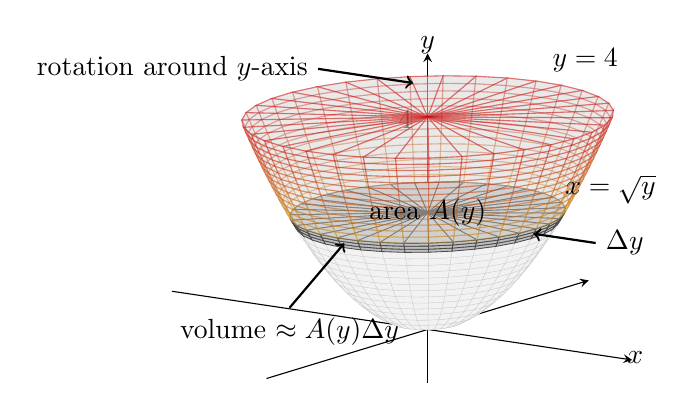
\begin{tikzpicture}
\begin{axis}[
    view={35}{20},
    width=0.95\textwidth,
    height=0.65\textwidth,
    grid=none,
    axis lines=center,
    xlabel={},
    ylabel={},
    zlabel={},
    ztick={0, 2, 2.2, 4},
    zticklabels={\(0\), \(y\), \(y+\Delta y\), \(4\)},
    xtick=\empty,
    ytick=\empty,
    xmin=-3.5, xmax=2.8,
    ymin=-2.8, ymax=2.8,
    zmin=-1.0, zmax=5.2,
    z buffer=sort
]

% 1. Back/Lower portion of the solid (y from 0 to 2)
\addplot3[
    surf,
    domain=0:2,
    y domain=0:360,
    samples=15,
    samples y=36,
    fill=gray!10,
    faceted color=gray!40,
    line width=0.1pt
] (
    {sqrt(x) * cos(y)}, % Radius function r = sqrt(y)
    {sqrt(x) * sin(y)},
    {x}
);

% 2. Solid cap at y=2 (Back wall of the slice)
\addplot3[
    surf,
    domain=0:1,
    y domain=0:360,
    samples=2,
    samples y=36,
    fill=gray!30,
    faceted color=gray!50,
    line width=0.1pt
] (
    {1.414 * x * cos(y)}, % Radius is exactly sqrt(2) \approx 1.414 at y=2
    {1.414 * x * sin(y)},
    {2}
);

% 3. The highlighted differential slice crust (y from 2 to 2.2)
\addplot3[
    surf,
    domain=2:2.2,
    y domain=0:360,
    samples=4,
    samples y=36,
    fill=gray!50,
    faceted color=black!70,
    line width=0.3pt
] (
    {sqrt(x) * cos(y)},
    {sqrt(x) * sin(y)},
    {x}
);

% 4. Solid cap at y=2.2 (Front face of the slice)
\addplot3[
    surf,
    domain=0:1,
    y domain=0:360,
    samples=2,
    samples y=36,
    fill=gray!40,
    faceted color=black!70,
    line width=0.3pt
] (
    {1.483 * x * cos(y)}, % Radius is approx sqrt(2.2) \approx 1.483 at y=2.2
    {1.483 * x * sin(y)},
    {2.2}
);

% 5. Front/Glass upper portion of the solid (y from 2.2 to 4) - TRANSPARENT
\addplot3[
    surf,
    domain=2.2:4,
    y domain=0:360,
    samples=15,
    samples y=36,
    fill=gray!30,
    draw=none, % No grid
    opacity=0.35 % See-through
] (
    {sqrt(x) * cos(y)},
    {sqrt(x) * sin(y)},
    {x}
);

% 6. End/Glass cap at y=4 - TRANSPARENT
\addplot3[
    surf,
    domain=0:1,
    y domain=0:360,
    samples=2,
    samples y=36,
    fill=gray!30,
    draw=none,
    opacity=0.35
] (
    {2 * x * cos(y)}, % Radius function sqrt(4) = 2
    {2 * x * sin(y)},
    {4}
);

% --- Annotations ---

% Axis labels corrected to the proper 3D mapping axes
\node[anchor=west] at (axis cs:2.6, 0, 0) {\(x\)};
\node[anchor=south] at (axis cs:0, 0, 5.0) {\(y\)};

% Thickness dimension pointing to the FRONT-RIGHT edge of the slice
\draw[thick, <-] (axis cs:1.45, 0, 2.1) -- (axis cs:2.3, 0, 2.1) node[right] {\(\Delta y\)};

% Area label directly on the visible face of the slice
\node at (axis cs:0, 0, 2.2) {area \(A(y)\)};

% Volume label pointing to the FRONT edge of the slice
\node[anchor=north] at (axis cs:0, -2.4, 1.2) {volume \(\approx A(y)\Delta y\)};
\draw[thick, <-] (axis cs:0, -1.45, 2.1) -- (axis cs:0, -2.4, 1.2);

% Top curve boundary label
\node[anchor=south west] at (axis cs:0, 2.0, 4.0) {\(y=4\)};

% Surface label cleanly anchored along the FRONT-RIGHT edge
\node[anchor=west] at (axis cs:1.75, 0, 3.0) {\(x=\sqrt{y}\)};

% Rotation label pulled closer to the center, and plot xmin expanded to give it room
\draw[thick, <-] (axis cs:-0.2, 0, 4.6) -- (axis cs:-1.5, 0, 4.6) node[left] {rotation around \(y\)-axis};

\end{axis}
\end{tikzpicture}
\caption{Rotating around the \(y\)-axis suggests horizontal slices and an integral in \(y\).}
\label{fig:disk-method-y-axis}
\end{figure}

\subsection{A slicing checklist}
\label{subsec:slicing-checklist}

Volumes by slicing become manageable when the setup is organized.

\begin{quote}
\textbf{Setting up a volume by slicing.}

\begin{enumerate}
\item Choose the slicing direction.
\item Identify the interval for the slicing variable.
\item Draw or describe a typical cross section.
\item Find its area \(A(x)\) or \(A(y)\).
\item Integrate the cross-sectional area over the slicing interval.
\end{enumerate}
\end{quote}

For \(x\)-slices,

\[
V=\int_a^b A(x)\,dx.
\]

For \(y\)-slices,

\[
V=\int_c^d A(y)\,dy.
\]

The notation changes, but the idea does not.

\[
\boxed{
\text{volume}=\int(\text{area of one slice})(\text{slice thickness}).
}
\]

\subsection{Where this points}
\label{subsec:volume-slicing-hook-shells}

Disks and washers come from slices perpendicular to the axis of rotation.  They are
excellent when the cross sections are easy.

But some rotations make washers awkward.  A vertical strip rotated around a vertical
axis does not make a washer.  It makes a thin cylindrical shell.

That gives a different small piece:

\[
(\text{circumference})(\text{height})(\text{thickness}).
\]

The next section builds that shell method from the same slicing idea.
\section{Cylindrical shells}
\label{sec:cylindrical-shells}

Disks and washers came from slices perpendicular to the axis of rotation.  A vertical
slice rotated around the \(x\)-axis made a disk or a washer.  A horizontal slice rotated
around the \(y\)-axis did the same.

But a slice can also be parallel to the axis of rotation.

Then it does not sweep out a disk.  It sweeps out a thin cylindrical shell.

The small piece changes shape again:

\[
\text{shell volume}
\approx
(\text{circumference})(\text{height})(\text{thickness}).
\]

This is the shell method.

\subsection{A thin shell unwrapped}
\label{subsec:thin-shell-unwrapped}

Imagine a very thin metal can with radius \(r\), height \(h\), and thickness
\(\Delta r\).  If we cut the side wall and flatten it, it becomes almost a rectangle.

The rectangle has height

\[
h
\]

and width approximately equal to the circumference of the shell:

\[
2\pi r.
\]

So its area is approximately

\[
2\pi r h.
\]

Multiplying by the thickness \(\Delta r\), the volume of the thin shell is approximately

\[
\boxed{
\Delta V\approx 2\pi r h\,\Delta r.
}
\]


The word ``approximately'' is doing honest work.  The outer surface of the shell has
a slightly larger circumference than the inner surface.  But when the thickness is very
small, the difference is very small.

For a shell with constant height \(h\), inner radius \(r\), and outer radius
\(r+\Delta r\), the exact volume is

\[
\pi(r+\Delta r)^2h-\pi r^2h.
\]

Expand:

\[
\pi h\bigl((r+\Delta r)^2-r^2\bigr)
=
\pi h(2r\Delta r+(\Delta r)^2).
\]

So

\[
\Delta V
=
2\pi r h\,\Delta r+\pi h(\Delta r)^2.
\]

The first term is the shell approximation.  The second term contains
\((\Delta r)^2\), which becomes negligible compared with \(\Delta r\) as the shell
gets thinner.

That is the same pattern we have seen before.  The integral keeps the first-order
small piece and lets the higher-order error disappear in the limit.

\subsection{The shell method formula}
\label{subsec:shell-method-formula}

Suppose a region is rotated around the \(y\)-axis.  A vertical strip at position \(x\)
has thickness \(dx\).  If the strip has height \(H(x)\), then after rotation it makes a
thin cylindrical shell.

Its radius is

\[
x,
\]

its circumference is

\[
2\pi x,
\]

its height is

\[
H(x),
\]

and its thickness is

\[
dx.
\]

So the small volume is

\[
dV=2\pi xH(x)\,dx.
\]

Adding all shells gives the volume.

\begin{quote}
\textbf{Shell method about the \(y\)-axis.}
If a region between \(x=a\) and \(x=b\) is rotated around the \(y\)-axis, and a vertical
strip has height \(H(x)\), then

\[
\boxed{
V=2\pi\int_a^b xH(x)\,dx
}
\]

provided \(x\ge0\) on the interval.
\end{quote}

In words:

\[
\boxed{
\text{volume}=\int(\text{circumference})(\text{height})(\text{thickness}).
}
\]

If the region is rotated around the vertical line

\[
x=c,
\]

then the radius is the distance from the strip to the axis:

\[
|x-c|.
\]

The shell formula becomes

\[
\boxed{
V=2\pi\int_a^b |x-c|\,H(x)\,dx.
}
\]

If \(x-c\) does not change sign on the interval, the absolute value is usually removed
by writing the radius as a positive expression.

\paragraph{Example: rotating a region under a parabola.}
Find the volume formed by rotating the region under

\[
y=4-x^2
\]

from \(x=0\) to \(x=2\) around the \(y\)-axis.

A vertical strip at position \(x\) has height

\[
H(x)=4-x^2.
\]

When rotated around the \(y\)-axis, it forms a shell with radius \(x\).  Therefore

\[
V=2\pi\int_0^2 x(4-x^2)\,dx.
\]

Compute:

\[
V
=
2\pi\int_0^2 (4x-x^3)\,dx.
\]

Thus

\[
V
=
2\pi\left(2x^2-\frac{x^4}{4}\right)\Big|_0^2.
\]

At \(x=2\),

\[
2x^2-\frac{x^4}{4}
=
8-\frac{16}{4}
=
8-4
=
4.
\]

So

\[
V=2\pi(4)=\boxed{8\pi}.
\]

\begin{figure}[h]
\centering
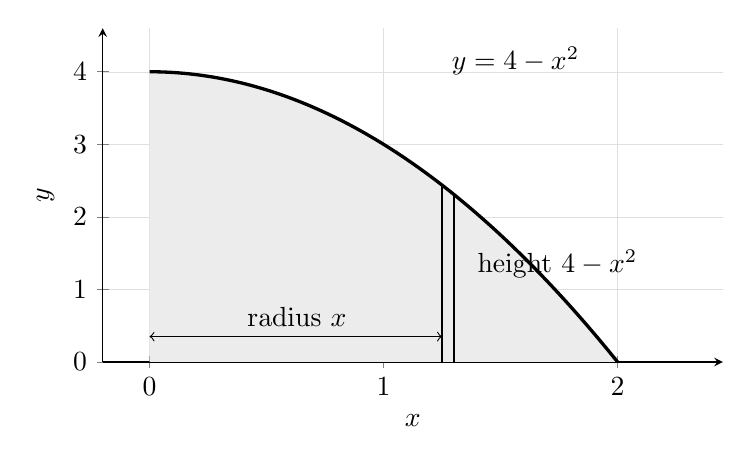
\begin{tikzpicture}
\begin{axis}[
    width=0.78\textwidth,
    height=0.48\textwidth,
    xmin=-0.2, xmax=2.45,
    ymin=0, ymax=4.6,
    axis lines=left,
    xlabel={\(x\)},
    ylabel={\(y\)},
    xtick={0,1,2},
    ytick={0,1,2,3,4},
    grid=both,
    grid style={line width=.1pt, draw=gray!25},
]
\addplot[domain=0:2, samples=120, fill=gray!15, draw=none] {4-x^2} \closedcycle;
\addplot[very thick, domain=0:2.15, samples=120] {4-x^2};

% typical shell-generating strip
\draw[thick] (axis cs:1.25,0) -- (axis cs:1.25,2.4375);
\draw[thick] (axis cs:1.30,0) -- (axis cs:1.30,2.31);
\draw[<->] (axis cs:0,0.35) -- (axis cs:1.25,0.35);
\node[above] at (axis cs:0.63,0.35) {radius \(x\)};
\node[anchor=west] at (axis cs:1.36,1.35) {height \(4-x^2\)};
\node[anchor=west] at (axis cs:1.25,4.15) {\(y=4-x^2\)};
\end{axis}
\end{tikzpicture}
\caption{A vertical strip rotated around the \(y\)-axis makes a cylindrical shell.}
\label{fig:shell-parabola}
\end{figure}

The shell formula is not a new principle.  It is the same slicing idea with a different
cross-sectional piece.

\subsection{When shells beat washers}
\label{subsec:when-shells-beat-washers}

The washer method uses slices perpendicular to the axis of rotation.  The shell method
uses slices parallel to the axis of rotation.

That one choice can turn a difficult setup into a simple one.

\begin{center}
\begin{tabular}{c|c|c}
\textbf{axis of rotation} & \textbf{slice direction} & \textbf{method} \\ \hline
vertical axis & horizontal slices & disks or washers \\
vertical axis & vertical slices & shells \\
horizontal axis & vertical slices & disks or washers \\
horizontal axis & horizontal slices & shells
\end{tabular}
\end{center}

A quick way to remember it is:

\[
\boxed{
\text{slices perpendicular to the axis make disks or washers;}
}
\]

\[
\boxed{
\text{slices parallel to the axis make shells.}
}
\]

\paragraph{Example: shells avoid splitting.}
Rotate the region under

\[
y=\frac1x
\]

from \(x=1\) to \(x=3\) around the \(y\)-axis.

With shells, a vertical strip has radius \(x\) and height \(\frac1x\).  So

\[
V=2\pi\int_1^3 x\cdot\frac1x\,dx.
\]

The factors cancel:

\[
V=2\pi\int_1^3 1\,dx
=
2\pi(3-1)
=
\boxed{4\pi}.
\]

\begin{figure}[h]
\centering
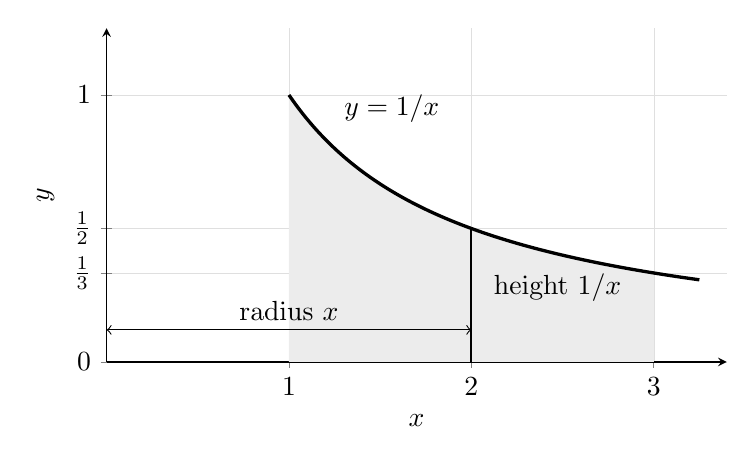
\begin{tikzpicture}
\begin{axis}[
    width=0.78\textwidth,
    height=0.48\textwidth,
    xmin=0, xmax=3.4,
    ymin=0, ymax=1.25,
    axis lines=left,
    xlabel={\(x\)},
    ylabel={\(y\)},
    xtick={1,2,3},
    ytick={0,0.333,0.5,1},
    yticklabels={\(0\),\(\frac13\),\(\frac12\),\(1\)},
    grid=both,
    grid style={line width=.1pt, draw=gray!25},
]
\addplot[domain=1:3, samples=120, fill=gray!15, draw=none] {1/x} \closedcycle;
\addplot[very thick, domain=1:3.25, samples=120] {1/x};
\draw[thick] (axis cs:2,0) -- (axis cs:2,0.5);
\draw[<->] (axis cs:0,0.12) -- (axis cs:2,0.12);
\node[above] at (axis cs:1,0.12) {radius \(x\)};
\node[anchor=west] at (axis cs:2.07,0.28) {height \(1/x\)};
\node[anchor=west] at (axis cs:1.25,0.95) {\(y=1/x\)};
\end{axis}
\end{tikzpicture}
\caption{The shell height is \(1/x\), so \(x\cdot(1/x)=1\).  The shell setup is especially simple.}
\label{fig:shell-1-over-x}
\end{figure}

Washers are possible, but they are less direct.  A horizontal slice must be described
in terms of \(y\).

The region has top value \(y=1\) and bottom value \(y=0\).  But the right boundary
changes its description:

\[
\begin{cases}
0\le y\le \frac13: & \text{the slice runs from }x=1\text{ to }x=3,\\[2mm]
\frac13<y\le 1: & \text{the slice runs from }x=1\text{ to }x=\frac1y.
\end{cases}
\]

So the washer method requires two integrals:

\[
V
=
\pi\int_0^{1/3}(3^2-1^2)\,dy
+
\pi\int_{1/3}^1\left(\left(\frac1y\right)^2-1^2\right)\,dy.
\]

This gives the same answer, but the shell method sees the region in one piece.

\[
\boxed{
\text{A good method is the one that describes the small piece simply.}
}
\]

\subsection{Comparing two methods on the same solid}
\label{subsec:comparing-shells-washers-same-solid}

Different methods should agree when they describe the same solid.  The setup may
look different, but the volume is the same physical quantity.

\paragraph{Example: rotating the region between \(y=x\) and \(y=x^2\).}
Rotate the region between

\[
y=x
\]

and

\[
y=x^2
\]

from \(x=0\) to \(x=1\) around the \(y\)-axis.

We compute the volume in two ways.

\subsubsection*{Shell method}

A vertical strip has radius

\[
x
\]

and height

\[
x-x^2.
\]

So

\[
V=2\pi\int_0^1 x(x-x^2)\,dx.
\]

Thus

\[
V=2\pi\int_0^1 (x^2-x^3)\,dx.
\]

Compute:

\[
V
=
2\pi\left(\frac{x^3}{3}-\frac{x^4}{4}\right)\Big|_0^1
=
2\pi\left(\frac13-\frac14\right)
=
2\pi\left(\frac1{12}\right).
\]

Therefore

\[
\boxed{
V=\frac{\pi}{6}.
}
\]

\subsubsection*{Washer method}

For washers about the \(y\)-axis, use horizontal slices.  Solve the curves for \(x\)
in terms of \(y\):

\[
y=x
\quad\Longrightarrow\quad
x=y,
\]

and

\[
y=x^2
\quad\Longrightarrow\quad
x=\sqrt y.
\]

For \(0\le y\le1\), the right boundary is \(x=\sqrt y\), and the left boundary is
\(x=y\).  Rotating around the \(y\)-axis gives washers with

\[
R(y)=\sqrt y,
\qquad
r(y)=y.
\]

Thus

\[
V=\pi\int_0^1\left((\sqrt y)^2-y^2\right)\,dy.
\]

So

\[
V=\pi\int_0^1 (y-y^2)\,dy.
\]

Compute:

\[
V
=
\pi\left(\frac{y^2}{2}-\frac{y^3}{3}\right)\Big|_0^1
=
\pi\left(\frac12-\frac13\right)
=
\boxed{\frac{\pi}{6}}.
\]

The two setups agree.

\begin{quote}
\textbf{The method is not the meaning.}

Shells and washers are two ways to add the same solid.  One adds thin cylindrical
walls.  The other adds thin cross-sectional washers.  If both describe the same solid
correctly, they give the same volume.
\end{quote}

\subsection{Shells around a horizontal axis}
\label{subsec:shells-horizontal-axis}

Shells are not only for rotation around the \(y\)-axis.  If a horizontal strip rotates
around a horizontal axis, it also makes a shell.

For example, suppose a region is described using \(y\), and a horizontal strip has
length \(L(y)\).  If the region is rotated around the \(x\)-axis, then the shell radius is
\(y\), the circumference is \(2\pi y\), and the thickness is \(dy\).

So

\[
\boxed{
V=2\pi\int_c^d yL(y)\,dy
}
\]

when \(y\ge0\).

More generally, rotating around the horizontal line \(y=k\) gives radius

\[
|y-k|.
\]

Then

\[
\boxed{
V=2\pi\int_c^d |y-k|\,L(y)\,dy.
}
\]

The same small piece is being used:

\[
(\text{circumference})(\text{height or length})(\text{thickness}).
\]

Only the variable changes.

\paragraph{Example: horizontal shells.}
Rotate the region between

\[
x=y^2
\]

and

\[
x=2-y^2
\]

for \(-1\le y\le1\) around the \(x\)-axis.

A horizontal strip at height \(y\) has length

\[
(2-y^2)-y^2=2-2y^2.
\]

But rotating the whole region around the \(x\)-axis using horizontal shells requires
care, because the strip above the \(x\)-axis and the strip below the \(x\)-axis make
the same shell radius.  If we integrate from \(-1\) to \(1\) using \(2\pi y\), the positive
and negative shell radii would cancel, which makes no physical sense.

Instead, use symmetry.  The upper half \((0\le y\le1)\) rotates to produce the whole
solid.  Its shell radius is \(y\).  Therefore

\[
V=2\pi\int_0^1 y(2-2y^2)\,dy.
\]

Compute:

\[
V=2\pi\int_0^1 (2y-2y^3)\,dy
=
2\pi\left(y^2-\frac{y^4}{2}\right)\Big|_0^1.
\]

So

\[
V=2\pi\left(1-\frac12\right)=\boxed{\pi}.
\]

\begin{quote}
\textbf{Warning.}
A radius is a distance, so it is nonnegative.  If a strip crosses the axis of rotation,
or if symmetric strips produce the same shell, split the region or use symmetry.
\end{quote}

Shells give one more way to choose the small piece.  The next section changes the
quantity being measured.  Instead of adding volume, we add matter.

\section{Mass, density, and center of mass}
\label{sec:mass-density-center-of-mass}

Area and volume assume the material is uniform.  But real objects are often heavier
in one place than another.

A metal rod may be denser near one end.  A wire may be made from two different
materials.  A thin plate may have paint or coating that varies from point to point.

Then length alone does not determine mass.  We need density.

The small piece becomes

\[
\text{small mass}=(\text{density})(\text{small length}).
\]

In symbols,

\[
dm=\lambda(x)\,dx.
\]

\subsection{Linear density and mass of a rod}
\label{subsec:linear-density-mass-rod}

Suppose a thin rod lies along the \(x\)-axis from \(x=a\) to \(x=b\).  Its density may
vary from point to point.

The \emph{linear density}

\[
\lambda(x)
\]

measures mass per unit length at position \(x\).

For example, if \(\lambda(x)\) is measured in grams per centimeter and \(dx\) is
measured in centimeters, then

\[
\lambda(x)\,dx
\]

has units

\[
\frac{\text{grams}}{\text{centimeter}}\cdot\text{centimeter}
=
\text{grams}.
\]

So the small mass is

\[
dm=\lambda(x)\,dx.
\]

Adding the small masses gives the total mass.

\begin{quote}
\textbf{Mass from linear density.}
If a rod lies from \(x=a\) to \(x=b\), and its linear density is \(\lambda(x)\), then its
mass is

\[
\boxed{
m=\int_a^b \lambda(x)\,dx.
}
\]
\end{quote}

This is the same accumulation idea again:

\[
\boxed{
\text{total mass}=\int(\text{mass per length})(\text{small length}).
}
\]

\paragraph{Example: a rod denser toward the right.}
A rod lies from \(x=0\) to \(x=4\) centimeters.  Its linear density is

\[
\lambda(x)=2+x
\]

grams per centimeter.  Find its mass.

The mass is

\[
m=\int_0^4 (2+x)\,dx.
\]

Compute:

\[
m=
\left(2x+\frac{x^2}{2}\right)\Big|_0^4
=
8+8
=
\boxed{16}
\]

grams.

The density is not constant.  Near \(x=0\), the density is \(2\) grams per centimeter.
Near \(x=4\), the density is \(6\) grams per centimeter.  The integral adds all the
varying small pieces of mass.

\begin{figure}[h]
\centering
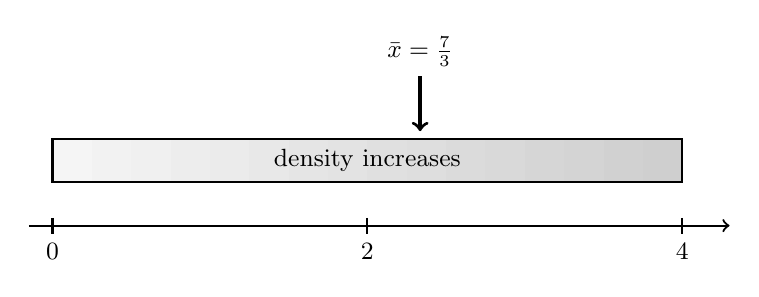
\begin{tikzpicture}[scale=1.0, every node/.style={font=\small}]
  % rod base
  \draw[thick] (0,0) rectangle (8,0.55);

  % simple density shading by strips
  \foreach \i in {0,...,15} {
    \pgfmathsetmacro{\shade}{8+2*\i}
    \fill[gray!\shade] ({0.5*\i},0) rectangle ({0.5*(\i+1)},0.55);
  }
  \draw[thick] (0,0) rectangle (8,0.55);

  % axis
  \draw[->, thick] (-0.3,-0.55) -- (8.6,-0.55);
  \foreach \x/\lab in {0/0,4/2,8/4} {
    \draw[thick] (\x,-0.45) -- (\x,-0.65);
    \node[below] at (\x,-0.65) {\(\lab\)};
  }

  % center of mass marker
  \draw[very thick, ->] (4.67,1.35) -- (4.67,0.65);
  \node[above] at (4.67,1.35) {\(\bar x=\frac73\)};

  \node at (4,0.28) {density increases};
\end{tikzpicture}
\caption{For \(\lambda(x)=2+x\) on \([0,4]\), more mass lies to the right, so the center of mass is right of the midpoint.}
\label{fig:rod-density-center-mass}
\end{figure}

\subsection{Moments}
\label{subsec:moments}

Mass tells how much matter there is.  It does not say where the matter is located.

To measure location, we use \emph{moments}.

Begin with point masses on a line.  Suppose masses

\[
m_1,m_2,\ldots,m_n
\]

are located at positions

\[
x_1,x_2,\ldots,x_n.
\]

The total mass is

\[
m=m_1+m_2+\cdots+m_n.
\]

The moment about the origin is

\[
M_0=m_1x_1+m_2x_2+\cdots+m_nx_n.
\]

A mass farther from the origin contributes more to the moment.  A mass on the
negative side contributes a negative moment.

\begin{quote}
\textbf{Moment of point masses on a line.}

\[
\boxed{
M_0=\sum_{i=1}^n m_i x_i.
}
\]
\end{quote}

The units are

\[
(\text{mass})(\text{length}).
\]

For a continuous rod, the small mass near \(x\) is

\[
dm=\lambda(x)\,dx.
\]

Its small moment about the origin is

\[
dM_0=x\,dm=x\lambda(x)\,dx.
\]

Adding gives

\[
\boxed{
M_0=\int_a^b x\lambda(x)\,dx.
}
\]

The moment is the mass-weighted accumulation of position.

\paragraph{Example: point masses.}
A mass of \(2\) kilograms is placed at \(x=1\), and a mass of \(6\) kilograms is placed
at \(x=5\).  The total mass is

\[
m=2+6=8.
\]

The moment about the origin is

\[
M_0=2(1)+6(5)=2+30=32.
\]

The heavier mass is farther to the right, so the moment is large and positive.

\subsection{Center of mass on a line}
\label{subsec:center-of-mass-line}

The center of mass is the balancing point.

For point masses, the balancing point \(\bar x\) should have the same total moment
as the whole system.  If all mass \(m\) were concentrated at \(\bar x\), its moment
would be

\[
m\bar x.
\]

So we require

\[
m\bar x=M_0.
\]

Therefore

\[
\boxed{
\bar x=\frac{M_0}{m}.
}
\]

For point masses,

\[
\boxed{
\bar x=
\frac{\sum_{i=1}^n m_i x_i}{\sum_{i=1}^n m_i}.
}
\]

For a continuous rod,

\[
m=\int_a^b \lambda(x)\,dx
\]

and

\[
M_0=\int_a^b x\lambda(x)\,dx.
\]

So

\[
\boxed{
\bar x
=
\frac{\int_a^b x\lambda(x)\,dx}{\int_a^b \lambda(x)\,dx}.
}
\]

This formula is a weighted average of position.  The weights are the small masses.

\paragraph{Example: center of mass of a nonuniform rod.}
Return to the rod on \([0,4]\) with density

\[
\lambda(x)=2+x.
\]

We already found its mass:

\[
m=16.
\]

Its moment about the origin is

\[
M_0=\int_0^4 x(2+x)\,dx.
\]

Compute:

\[
M_0=\int_0^4 (2x+x^2)\,dx
=
\left(x^2+\frac{x^3}{3}\right)\Big|_0^4.
\]

Thus

\[
M_0=16+\frac{64}{3}=\frac{112}{3}.
\]

Therefore

\[
\bar x=\frac{M_0}{m}
=
\frac{\frac{112}{3}}{16}
=
\frac{112}{48}
=
\boxed{\frac73}.
\]

So the center of mass is at

\[
x=\frac73\approx2.33.
\]

The midpoint of the rod is \(2\).  The center of mass is farther to the right because
the rod is denser there.

\paragraph{Example: symmetry can find the center.}
Let a rod lie from \(x=-1\) to \(x=1\), with density

\[
\lambda(x)=1+x^2.
\]

This density is symmetric:

\[
\lambda(-x)=\lambda(x).
\]

So the left half and right half balance.  The center of mass should be

\[
\bar x=0.
\]

The moment confirms this:

\[
M_0=\int_{-1}^1 x(1+x^2)\,dx.
\]

The integrand

\[
x(1+x^2)=x+x^3
\]

is odd.  The integral of an odd function over a symmetric interval is \(0\).  Hence

\[
M_0=0.
\]

Since the total mass is positive,

\[
\bar x=\frac{0}{m}=0.
\]

Symmetry is not a trick.  It is a way of seeing cancellation before calculating.

\begin{quote}
\textbf{Warning.}
The center of mass formula requires positive total mass.  Ordinary densities are
nonnegative, so this is usually automatic.  If signed ``masses'' are allowed and the
total mass is \(0\), then

\[
\bar x=\frac{M_0}{m}
\]

has no meaning.  A balancing point for physical mass comes from positive mass.
\end{quote}

\subsection{Uniform density as a check}
\label{subsec:uniform-density-check}

If density is constant, the center of mass should be the geometric midpoint.

Suppose

\[
\lambda(x)=\lambda_0
\]

on \([a,b]\), where \(\lambda_0>0\).  Then

\[
m=\int_a^b \lambda_0\,dx=\lambda_0(b-a).
\]

The moment is

\[
M_0=\int_a^b x\lambda_0\,dx
=
\lambda_0\left(\frac{x^2}{2}\right)\Big|_a^b
=
\lambda_0\frac{b^2-a^2}{2}.
\]

So

\[
\bar x
=
\frac{\lambda_0\frac{b^2-a^2}{2}}{\lambda_0(b-a)}.
\]

Cancel \(\lambda_0\), and factor

\[
b^2-a^2=(b-a)(b+a).
\]

Then

\[
\bar x
=
\frac{(b-a)(b+a)}{2(b-a)}
=
\boxed{\frac{a+b}{2}}.
\]

The formula passes the basic test.  A uniform rod balances at its midpoint.

\subsection{A lamina preview by slices}
\label{subsec:lamina-preview-slices}

A \emph{lamina} is a thin flat plate.  Its mass depends on area density, not linear
density.

If the areal density is

\[
\sigma
\]

with units mass per unit area, then

\[
dm=\sigma\,dA.
\]

A full treatment belongs to multivariable calculus.  But many lamina problems can
already be handled by slicing.

Suppose a plate lies between

\[
y=b(x)
\]

and

\[
y=t(x)
\]

for

\[
a\le x\le b,
\]

and suppose its areal density \(\sigma(x)\) is constant along each vertical slice.  A
vertical slice has height

\[
t(x)-b(x)
\]

and thickness

\[
dx.
\]

So its area is approximately

\[
dA=(t(x)-b(x))\,dx.
\]

Its mass is

\[
dm=\sigma(x)(t(x)-b(x))\,dx.
\]

Therefore the total mass is

\[
\boxed{
m=\int_a^b \sigma(x)(t(x)-b(x))\,dx.
}
\]

The moment about the \(y\)-axis uses the horizontal position \(x\):

\[
\boxed{
M_y=\int_a^b x\,\sigma(x)(t(x)-b(x))\,dx.
}
\]

So

\[
\boxed{
\bar x=\frac{M_y}{m}.
}
\]

If the density is uniform along each vertical slice, then the vertical center of that
slice is halfway between its bottom and top:

\[
\frac{b(x)+t(x)}{2}.
\]

The moment about the \(x\)-axis is

\[
\boxed{
M_x=\int_a^b
\frac{b(x)+t(x)}{2}\,
\sigma(x)(t(x)-b(x))\,dx.
}
\]

Then

\[
\boxed{
\bar y=\frac{M_x}{m}.
}
\]

These formulas are still one-variable integrals because each slice has been reduced
to one small mass placed at the slice's own center.

\paragraph{Example: center of mass of a triangular lamina.}
Find the center of mass of the triangular plate bounded by

\[
y=0,\qquad y=x,\qquad x=2,
\]

assuming constant areal density \(\sigma\).

A vertical slice at \(x\) runs from \(y=0\) to \(y=x\).  Its height is

\[
x.
\]

So

\[
dm=\sigma x\,dx,
\qquad 0\le x\le2.
\]

The mass is

\[
m=\int_0^2 \sigma x\,dx
=
\sigma\left(\frac{x^2}{2}\right)\Big|_0^2
=
2\sigma.
\]

The moment about the \(y\)-axis is

\[
M_y=\int_0^2 x(\sigma x)\,dx
=
\sigma\int_0^2 x^2\,dx.
\]

Thus

\[
M_y
=
\sigma\left(\frac{x^3}{3}\right)\Big|_0^2
=
\frac{8\sigma}{3}.
\]

So

\[
\bar x=\frac{M_y}{m}
=
\frac{\frac{8\sigma}{3}}{2\sigma}
=
\boxed{\frac43}.
\]

For the vertical coordinate, each slice has midpoint height

\[
\frac{x}{2}.
\]

So the small moment about the \(x\)-axis is

\[
dM_x=\frac{x}{2}\,dm
=
\frac{x}{2}\sigma x\,dx.
\]

Therefore

\[
M_x=\int_0^2 \frac{\sigma x^2}{2}\,dx
=
\frac{\sigma}{2}\left(\frac{x^3}{3}\right)\Big|_0^2
=
\frac{4\sigma}{3}.
\]

Thus

\[
\bar y=\frac{M_x}{m}
=
\frac{\frac{4\sigma}{3}}{2\sigma}
=
\boxed{\frac23}.
\]

The center of mass is

\[
\boxed{
\left(\frac43,\frac23\right).
}
\]

\begin{figure}[h]
\centering
\begin{tikzpicture}[scale=2.15, every node/.style={font=\small}]
  % axes
  \draw[->, thick] (-0.2,0) -- (2.6,0);
  \draw[->, thick] (0,-0.2) -- (0,2.45);
  \node[right] at (2.6,0) {\(x\)};
  \node[above] at (0,2.45) {\(y\)};

  % triangle
  \fill[gray!15] (0,0) -- (2,0) -- (2,2) -- cycle;
  
  % white slice fill with slanted mesh lines
  \fill[blue] (1.25,0) -- (1.32,0) -- (1.32,1.32) -- (1.25,1.25) -- cycle;
  \fill[pattern=north east lines, pattern color=red!80] (1.25,0) -- (1.32,0) -- (1.32,1.32) -- (1.25,1.25) -- cycle;
  
  \draw[very thick] (0,0) -- (2,2);
  \draw[very thick] (2,0) -- (2,2);
  \draw[very thick] (0,0) -- (2,0);

  % vertical slice borders
  \draw[thick] (1.25,0) -- (1.25,1.25);
  \draw[thick] (1.32,0) -- (1.32,1.32);

  % slice height brace
  \draw[decorate, decoration={brace, amplitude=3pt}] 
    (1.35,1.32) -- (1.35,0) 
    node[midway, right=3pt] {slice height \(x\)};

  % center of mass
  \fill (1.333,0.667) circle (1.3pt);
  \node[anchor=east] at (1.32,0.67) {\(\left(\frac43,\frac23\right)\)};

  % labels
  \node[below] at (2,0) {\(2\)};
  \node[left] at (0,2) {\(2\)};
  \node[anchor=west] at (0.7,1.55) {\(y=x\)};
\end{tikzpicture}
\caption{A triangular lamina can be handled by vertical slices.  Each slice contributes mass and moment.}
\label{fig:triangular-lamina-center-mass}
\end{figure}

The density \(\sigma\) canceled from the center of mass because it was constant.  If the
density varied, it would not usually cancel.

\subsection{What center of mass is measuring}
\label{subsec:what-center-of-mass-measures}

The center of mass is not the geometric center unless mass is spread uniformly.

It is the average location of mass.

For a rod,

\[
\bar x
=
\frac{\int_a^b x\lambda(x)\,dx}{\int_a^b \lambda(x)\,dx}.
\]

The denominator adds the mass.  The numerator adds position weighted by mass.

For a lamina,

\[
\bar x
=
\frac{M_y}{m},
\qquad
\bar y
=
\frac{M_x}{m}.
\]

The notation looks backwards at first: \(M_y\) gives \(\bar x\), and \(M_x\) gives
\(\bar y\).  The reason is that \(M_y\) is the moment about the \(y\)-axis, so it uses
horizontal distance from that axis.  That horizontal distance is \(x\).  Similarly,
\(M_x\) uses vertical distance \(y\).

\begin{quote}
\textbf{Mass and moment small pieces.}

For a rod:

\[
dm=\lambda(x)\,dx,
\qquad
dM_0=x\,dm.
\]

For a sliced lamina:

\[
dm=\sigma(x)(\text{slice height})\,dx,
\qquad
dM_y=x\,dm.
\]

The pattern is always the same:

\[
\text{moment}=(\text{distance from axis})(\text{mass}).
\]
\end{quote}

Mass asks:

\[
\text{How much matter is there?}
\]

Moment asks:

\[
\text{Where is that matter, with respect to an axis?}
\]

Center of mass combines the two:

\[
\text{Where could all the mass be placed to have the same moment?}
\]

The next application changes the physical meaning again.  Instead of adding small
masses, we will add small amounts of work:

\[
dW=F(x)\,dx.
\]

The small piece is force times displacement.  The integral will measure energy transferred
through motion.
\section{Work and energy}
\label{sec:work-energy}

The last section added small pieces of mass:

\[
dm=\lambda(x)\,dx.
\]

Now the quantity changes again.  A force moves an object through a distance.  The small
piece is

\[
dW=F(x)\,dx.
\]

This accumulated quantity is called \emph{work}.  It measures energy transferred by a
force through motion.

\subsection{Constant force and variable force}
\label{subsec:constant-variable-force}

If a constant force moves an object in the same direction as the motion, the work is

\[
\text{work}=(\text{force})(\text{distance}).
\]

For example, if a force of \(10\) newtons pushes a box \(3\) meters, then the work done is

\[
10\cdot 3=30
\]

newton-meters.

A newton-meter is called a \emph{joule}.  So the work is

\[
30\text{ joules}.
\]

In symbols,

\[
W=Fd.
\]

This is the same kind of formula as

\[
\text{distance}=(\text{velocity})(\text{time}).
\]

It is exact when the force is constant.

But forces are often not constant.  A spring pulls harder the more it is stretched.  A rope
or chain may require more work to lift one part than another.  Water in a tank must be
lifted different distances depending on where the water is.

So we return to the same idea:

\[
\boxed{
\text{break the motion into small pieces, estimate the work on each piece, and add.}
}
\]

Suppose an object moves along the \(x\)-axis from \(x=a\) to \(x=b\), and a force \(F(x)\)
acts in the direction of motion.  On a short interval of length \(\Delta x\), the force is
approximately constant, so

\[
\Delta W\approx F(x)\Delta x.
\]

Adding and taking the limit gives the work.

\begin{quote}
\textbf{Work by a variable force.}
If \(F(x)\) is a continuous force acting along the \(x\)-axis as an object moves from
\(x=a\) to \(x=b\), then the work done is

\[
\boxed{
W=\int_a^b F(x)\,dx.
}
\]
\end{quote}

In words:

\[
\boxed{
\text{work}=\int(\text{force})(\text{small displacement}).
}
\]

The units check the meaning.  If \(F(x)\) is measured in newtons and \(x\) in meters, then

\[
F(x)\,dx
\]

has units

\[
\text{newtons}\cdot\text{meters}=\text{joules}.
\]

\paragraph{Example: a force that increases with position.}
A force is given by

\[
F(x)=5+2x
\]

newtons, where \(x\) is measured in meters.  Find the work done as an object moves
from \(x=0\) to \(x=3\).

The work is

\[
W=\int_0^3 (5+2x)\,dx.
\]

Compute:

\[
W=
\left(5x+x^2\right)\Big|_0^3
=
15+9
=
\boxed{24}
\]

joules.

\begin{figure}[h]
\centering
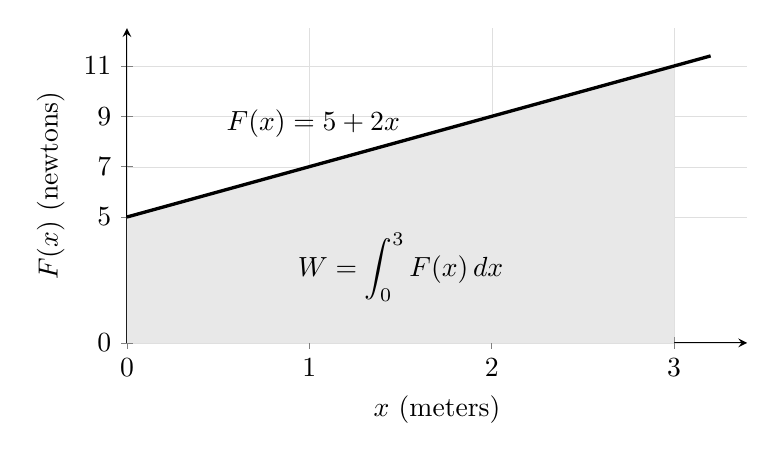
\begin{tikzpicture}
\begin{axis}[
    width=0.78\textwidth,
    height=0.46\textwidth,
    xmin=0, xmax=3.4,
    ymin=0, ymax=12.5,
    axis lines=left,
    xlabel={\(x\) (meters)},
    ylabel={\(F(x)\) (newtons)},
    xtick={0,1,2,3},
    ytick={0,5,7,9,11},
    grid=both,
    grid style={line width=.1pt, draw=gray!25},
]
\addplot[domain=0:3, samples=2, fill=gray!18, draw=none] {5+2*x} \closedcycle;
\addplot[very thick, domain=0:3.2, samples=2] {5+2*x};
\node[anchor=east] at (axis cs:1.55,8.7) {\(F(x)=5+2x\)};
\node at (axis cs:1.5,3.0) {\(W=\displaystyle\int_0^3 F(x)\,dx\)};
\end{axis}
\end{tikzpicture}
\caption{Work is the accumulated area under a force-versus-position graph.}
\label{fig:work-force-area}
\end{figure}

\paragraph{A warning about final force.}
If

\[
F(x)=x
\]

on \(0\le x\le2\), then the final force is

\[
F(2)=2.
\]

Multiplying final force by total distance gives

\[
2\cdot2=4.
\]

But the actual work is

\[
\int_0^2 x\,dx
=
\left(\frac{x^2}{2}\right)\Big|_0^2
=
2.
\]

The final force acted only at the end.  It did not act for the whole motion.

\begin{quote}
\textbf{Warning.}
For a variable force, do not use

\[
(\text{final force})(\text{total distance})
\]

unless the force really was constant.  The integral adds the changing force over the
whole path.
\end{quote}

\paragraph{Signed work.}
Work can be negative.  If the force points opposite the direction of motion, then
\(F(x)<0\), and

\[
\int_a^b F(x)\,dx
\]

is negative.  Negative work means the force removes energy from the moving object
rather than adding energy to it.

For now, most examples use positive forces in the direction of motion.  The sign is
still part of the formula.

\subsection{Springs and Hooke's law}
\label{subsec:springs-hookes-law}

A spring gives the first natural example of a variable force.

When a spring is at its natural length, it does not need any force to hold it there.
When it is stretched, it pulls back.  For many springs, at ordinary stretches, the force
needed to hold the spring stretched \(x\) units is proportional to \(x\):

\[
F(x)=kx.
\]

The constant \(k\) is called the \emph{spring constant}.  This relation is called
\emph{Hooke's law}.

A stiffer spring has a larger \(k\).  It takes more force to stretch it the same distance.

\begin{quote}
\textbf{Hooke's law.}
If a spring has spring constant \(k\), then the force needed to hold it stretched
\(x\) units beyond its natural length is

\[
\boxed{
F(x)=kx.
}
\]
\end{quote}

The work to stretch the spring from \(x=0\) to \(x=a\) is

\[
W=\int_0^a kx\,dx.
\]

Thus

\[
W
=
k\left(\frac{x^2}{2}\right)\Big|_0^a
=
\boxed{\frac12ka^2}.
\]

The factor \(\frac12\) appears because the force starts at \(0\) and grows linearly.

\begin{figure}[h]
\centering
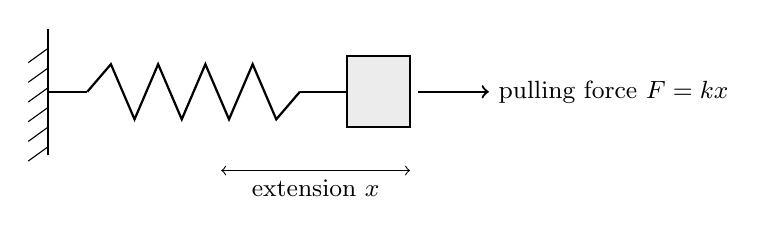
\begin{tikzpicture}[scale=1.0, every node/.style={font=\small}]
  % wall
  \draw[thick] (0,-0.8) -- (0,0.8);
  \foreach \y in {-0.7,-0.45,...,0.7} {
    \draw (0,\y) -- (-0.25,\y-0.18);
  }

  % spring zigzag
  \draw[thick] (0,0) -- (0.5,0);
  \draw[thick]
    (0.5,0) -- (0.8,0.35) -- (1.1,-0.35) -- (1.4,0.35) -- (1.7,-0.35)
    -- (2.0,0.35) -- (2.3,-0.35) -- (2.6,0.35) -- (2.9,-0.35)
    -- (3.2,0);
  \draw[thick] (3.2,0) -- (3.8,0);

  % block
  \draw[fill=gray!15, thick] (3.8,-0.45) rectangle (4.6,0.45);

  % extension arrow
  \draw[<->] (2.2,-1.0) -- (4.6,-1.0);
  \node[below] at (3.4,-1.0) {extension \(x\)};

  % force arrow
  \draw[->, thick] (4.7,0) -- (5.6,0);
  \node[right] at (5.6,0) {pulling force \(F=kx\)};
\end{tikzpicture}
\caption{The farther the spring is stretched, the larger the force needed to hold it.}
\label{fig:spring-hookes-law}
\end{figure}

\paragraph{Example: stretching a spring.}
A spring has spring constant

\[
k=200
\]

newtons per meter.  How much work is required to stretch it from its natural length
to \(0.20\) meters beyond its natural length?

The force needed at extension \(x\) is

\[
F(x)=200x.
\]

So

\[
W=\int_0^{0.20} 200x\,dx.
\]

Compute:

\[
W=
100x^2\Big|_0^{0.20}
=
100(0.20)^2
=
100(0.04)
=
\boxed{4}
\]

joules.

\paragraph{Example: stretching farther from an already stretched position.}
The same spring is already stretched \(0.20\) meters.  How much additional work is
required to stretch it to \(0.50\) meters beyond its natural length?

Now the interval is

\[
0.20\le x\le0.50.
\]

The work is

\[
W=\int_{0.20}^{0.50} 200x\,dx.
\]

Thus

\[
W=100x^2\Big|_{0.20}^{0.50}
=
100\left(0.50^2-0.20^2\right).
\]

So

\[
W=100(0.25-0.04)=\boxed{21}
\]

joules.

Stretching from \(0.20\) to \(0.50\) meters takes more work than stretching from
\(0\) to \(0.20\), because the spring is already pulling harder.

\begin{quote}
\textbf{Warning.}
In Hooke's law, \(x\) is the extension from the natural length, not necessarily the
total length of the spring.

If a spring has natural length \(10\) cm and is stretched to length \(18\) cm, then the
extension is \(8\) cm, not \(18\) cm.
\end{quote}

\subsection{Lifting a chain}
\label{subsec:lifting-chain}

A chain gives another example where different pieces require different amounts of work.

Imagine a chain of length \(L\) hanging vertically from the edge of a roof.  We want to
pull the whole chain up to the roof.

The top part of the chain travels only a short distance.  The bottom part travels a long
distance.  So one formula for the whole chain is not visible at first.  We slice the chain
into small pieces.

Let

\[
\lambda
\]

be the weight density of the chain, measured in pounds per foot or newtons per meter.
Let \(y\) measure distance below the roof.  A small piece of chain of length \(dy\) at
distance \(y\) below the roof has weight

\[
\lambda\,dy.
\]

To reach the roof, that piece must be lifted distance

\[
y.
\]

So the small work is

\[
dW=(\lambda\,dy)y.
\]

That is,

\[
dW=\lambda y\,dy.
\]

Adding all pieces from \(y=0\) to \(y=L\),

\[
W=\int_0^L \lambda y\,dy.
\]

Thus

\[
W
=
\lambda\left(\frac{y^2}{2}\right)\Big|_0^L
=
\boxed{\frac12\lambda L^2}.
\]

\begin{figure}[h]
\centering
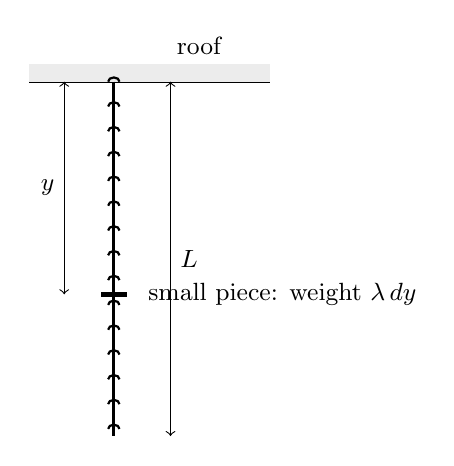
\begin{tikzpicture}[scale=0.9, every node/.style={font=\small}]
  % roof
  \draw[thick] (-1.2,0) -- (2.2,0);
  \fill[gray!15] (-1.2,0) rectangle (2.2,0.25);
  \node[above] at (1.2,0.25) {roof};

  % hanging chain
  \draw[very thick] (0,0) -- (0,-5);
  \foreach \y in {0,-0.35,...,-5} {
    \draw[thick] (-0.08,\y) arc[start angle=180,end angle=0,x radius=0.08,y radius=0.06];
  }

  % slice
  \draw[line width=2pt] (-0.18,-3.0) -- (0.18,-3.0);
  \node[right] at (0.35,-3.0) {small piece: weight \(\lambda\,dy\)};

  % depth arrow
  \draw[<->] (-0.7,0) -- (-0.7,-3.0);
  \node[left] at (-0.7,-1.5) {\(y\)};

  % length arrow
  \draw[<->] (0.8,0) -- (0.8,-5);
  \node[right] at (0.8,-2.5) {\(L\)};
\end{tikzpicture}
\caption{A piece \(y\) units below the roof must be lifted \(y\) units.}
\label{fig:lifting-chain}
\end{figure}

\paragraph{Example.}
A \(10\)-foot chain weighs \(2\) pounds per foot.  How much work is required to pull
the entire hanging chain up to the roof?

Here

\[
L=10,
\qquad
\lambda=2.
\]

So

\[
W=\int_0^{10} 2y\,dy.
\]

Compute:

\[
W=
y^2\Big|_0^{10}
=
\boxed{100}
\]

foot-pounds.

The unit is foot-pound because the force is measured in pounds and the distance in feet.

\paragraph{Why not weight times full length?}
The chain's total weight is

\[
2\cdot10=20
\]

pounds.  Multiplying by the full length gives

\[
20\cdot10=200
\]

foot-pounds.

That is too large.  It treats every piece as if it were lifted \(10\) feet.  But the top
pieces move less than \(10\) feet.  The integral correctly weights each piece by its own
lifting distance.

For a uniform hanging chain, the average lifting distance is \(L/2\).  Thus the total work is

\[
(\text{total weight})\left(\frac{L}{2}\right),
\]

which agrees with

\[
\frac12\lambda L^2.
\]

\subsection{Pumping fluid from a tank}
\label{subsec:pumping-fluid-tank}

Pumping fluid combines the chain idea with volume slicing.

Each thin layer of fluid has a weight.  Each layer must be lifted a certain distance.
The work for one layer is

\[
(\text{weight of layer})(\text{lifting distance}).
\]

Let

\[
\gamma
\]

be the weight density of the fluid.  For water,

\[
\gamma\approx62.4\text{ lb/ft}^3
\]

in English units, and

\[
\gamma\approx9800\text{ N/m}^3
\]

in metric units.

Suppose a horizontal slice of fluid at height \(y\) has cross-sectional area

\[
A(y).
\]

If the slice has thickness \(dy\), then its volume is approximately

\[
A(y)\,dy.
\]

Its weight is

\[
\gamma A(y)\,dy.
\]

If that slice must be lifted distance \(D(y)\), then

\[
dW=\gamma A(y)D(y)\,dy.
\]

Therefore

\[
\boxed{
W=\int \gamma A(y)D(y)\,dy.
}
\]

The limits come from the vertical range of the fluid.

\paragraph{Example: pumping out a rectangular tank.}
A rectangular tank is \(6\) feet long, \(4\) feet wide, and \(5\) feet deep.  It is full of
water.  How much work is required to pump all the water over the top edge?

Let \(y\) measure height above the bottom of the tank.  Then

\[
0\le y\le5.
\]

A horizontal slice has area

\[
A(y)=6\cdot4=24
\]

square feet.

A slice at height \(y\) must be lifted to the top, so its lifting distance is

\[
D(y)=5-y.
\]

The small work is

\[
dW=62.4\cdot24(5-y)\,dy.
\]

Thus

\[
W=62.4\int_0^5 24(5-y)\,dy.
\]

Compute:

\[
W=62.4\cdot24\left(5y-\frac{y^2}{2}\right)\Big|_0^5.
\]

Since

\[
5(5)-\frac{25}{2}
=
25-\frac{25}{2}
=
\frac{25}{2},
\]

we get

\[
W=62.4\cdot24\cdot\frac{25}{2}.
\]

Thus

\[
W=\boxed{18{,}720}
\]

foot-pounds.

\begin{figure}[h]
\centering
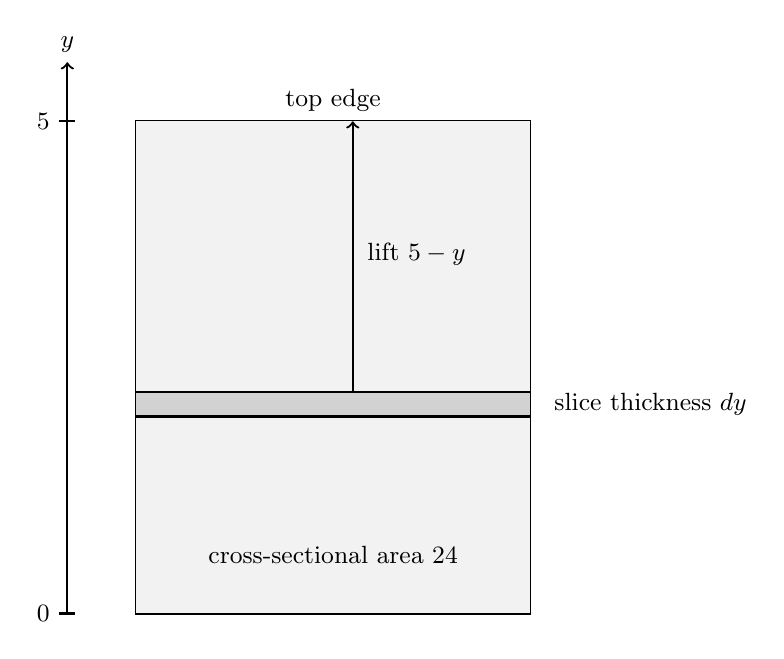
\begin{tikzpicture}[scale=1.25, every node/.style={font=\small}]
  % Tank outline
  \draw[thick] (0,0) rectangle (4,5);
  \fill[gray!10] (0,0) rectangle (4,5);

  % water slice
  \fill[gray!35] (0,2) rectangle (4,2.25);
  \draw[thick] (0,2) -- (4,2);
  \draw[thick] (0,2.25) -- (4,2.25);
  \node[right] at (4.15,2.12) {slice thickness \(dy\)};

  % coordinate axis
  \draw[->, thick] (-0.7,0) -- (-0.7,5.6);
  \node[above] at (-0.7,5.6) {\(y\)};
  \foreach \y/\lab in {0/0,5/5} {
    \draw[thick] (-0.78,\y) -- (-0.62,\y);
    \node[left] at (-0.78,\y) {\(\lab\)};
  }

  % lift arrow
  \draw[->, thick] (2.2,2.25) -- (2.2,5);
  \node[right] at (2.25,3.65) {lift \(5-y\)};

  \node[above] at (2,5) {top edge};
  \node at (2,0.6) {cross-sectional area \(24\)};
\end{tikzpicture}
\caption{Each water slice has the same area, but the lower slices must be lifted farther.}
\label{fig:pumping-rectangular-tank}
\end{figure}

\paragraph{Example: pumping out a conical tank.}
A conical tank has height \(6\) feet and radius \(3\) feet at the top.  Its vertex is at
the bottom.  It is full of water.  Find the work required to pump all the water over the
top.

Let \(y\) measure height above the bottom.  Then

\[
0\le y\le6.
\]

At height \(y\), the radius of the water slice is found by similar triangles:

\[
\frac{r(y)}{y}=\frac{3}{6}=\frac12.
\]

So

\[
r(y)=\frac{y}{2}.
\]

The area of the horizontal slice is

\[
A(y)=\pi r(y)^2
=
\pi\left(\frac{y}{2}\right)^2
=
\frac{\pi y^2}{4}.
\]

The slice must be lifted to the top, so

\[
D(y)=6-y.
\]

Thus

\[
W=62.4\int_0^6 \frac{\pi y^2}{4}(6-y)\,dy.
\]

Factor out constants:

\[
W=\frac{62.4\pi}{4}\int_0^6 (6y^2-y^3)\,dy.
\]

Compute the integral:

\[
\int_0^6 (6y^2-y^3)\,dy
=
\left(2y^3-\frac{y^4}{4}\right)\Big|_0^6.
\]

At \(y=6\),

\[
2(6^3)-\frac{6^4}{4}
=
432-324
=
108.
\]

So

\[
W=\frac{62.4\pi}{4}\cdot108
=
62.4\cdot27\pi.
\]

Therefore

\[
\boxed{
W=1684.8\pi
}
\]

foot-pounds.

\begin{quote}
\textbf{Pumping checklist.}

\begin{enumerate}
\item Choose a vertical coordinate.
\item Find the area \(A(y)\) of a horizontal slice.
\item Find the lifting distance \(D(y)\).
\item Write

\[
dW=\gamma A(y)D(y)\,dy.
\]

\item Integrate over the fluid's vertical range.
\end{enumerate}
\end{quote}

Pumping problems are work problems.  The only new step is geometric: finding the
volume of one thin layer.

\subsection{Energy stored by work}
\label{subsec:energy-stored-by-work}

Work transfers energy.

When we stretch a spring, the work we do is stored as elastic potential energy.  When we
lift a chain, the work becomes gravitational potential energy.  When we pump water up
and out of a tank, the work raises the water.

This is why work appears so often in physics and engineering.  A force acting through a
distance can change the energy of a system.

For this chapter, the calculus point is the same as before:

\[
\boxed{
\text{work is accumulated force over distance.}
}
\]

The next problem still involves water, but the water does not move.  It simply pushes.
The force from still water is not the same at every depth.  Deeper water pushes harder.

That gives a new small piece:

\[
dF=(\text{pressure at depth})(\text{small area}).
\]

\section{Hydrostatic force}
\label{sec:hydrostatic-force}

Pumping water asked how much work is needed to move water.  A dam or a window in
a tank asks a different question:

\[
\text{How hard does still water push?}
\]

The force is not spread evenly.  Near the surface, the water pressure is small.  Deep below
the surface, the pressure is larger.

So the small piece changes again:

\[
dF=(\text{pressure})(\text{small area}).
\]

\subsection{Pressure depends on depth}
\label{subsec:pressure-depth}

Pressure means force per unit area:

\[
\text{pressure}=\frac{\text{force}}{\text{area}}.
\]

If force is measured in pounds and area in square feet, pressure is measured in

\[
\text{lb/ft}^2.
\]

If force is measured in newtons and area in square meters, pressure is measured in

\[
\text{N/m}^2.
\]

A fluid at rest has pressure that increases with depth.  Let

\[
\gamma
\]

be the weight density of the fluid.  At depth \(h\), the pressure due to the fluid is

\[
\boxed{
p=\gamma h.
}
\]

Here \(h\) is measured downward from the fluid surface.

Why is this reasonable?  Imagine a column of water with cross-sectional area \(A\) and
height \(h\).  Its volume is

\[
Ah.
\]

Its weight is

\[
\gamma Ah.
\]

That weight is supported by area \(A\), so the pressure is

\[
\frac{\gamma Ah}{A}=\gamma h.
\]

\begin{quote}
\textbf{Hydrostatic pressure.}
At depth \(h\) below the surface of a fluid with weight density \(\gamma\), the pressure
due to the fluid is

\[
\boxed{
p(h)=\gamma h.
}
\]
\end{quote}

This is gauge pressure: pressure from the fluid above the point.  Atmospheric pressure
usually acts on both sides of a wall or plate, so in many hydrostatic-force problems it
cancels and is not included.

\paragraph{Example: pressure in a pool.}
Water has weight density approximately

\[
62.4\text{ lb/ft}^3.
\]

At depth \(8\) feet, the pressure due to the water is

\[
p=62.4(8)=499.2
\]

pounds per square foot.

At depth \(3\) feet, the pressure is

\[
p=62.4(3)=187.2
\]

pounds per square foot.

The deeper point has greater pressure because more water lies above it.

\begin{quote}
\textbf{Pressure is not total force.}
Pressure is force per unit area.  To find total force, multiply pressure by area only when
the pressure is constant over that area.

On a vertical wall, pressure changes with depth, so we must integrate.
\end{quote}

\subsection{Force on a vertical plate}
\label{subsec:force-vertical-plate}

A vertical plate in water feels different pressure at different depths.  Horizontal strips
solve the problem because each thin horizontal strip has nearly one depth.

\paragraph{Example: a rectangular plate.}
A rectangular plate is \(4\) feet wide and \(6\) feet high.  It stands vertically in water
with its top edge at the water surface.  Find the force of the water on the plate.

Let \(y\) be depth below the surface.  Then

\[
0\le y\le6.
\]

At depth \(y\), the pressure is

\[
p(y)=62.4y.
\]

A thin horizontal strip has width \(4\) feet and thickness \(dy\), so its area is

\[
4\,dy.
\]

The force on this strip is approximately

\[
dF=p(y)(4\,dy).
\]

Thus

\[
dF=62.4y\cdot4\,dy.
\]

Integrate from \(0\) to \(6\):

\[
F=62.4\int_0^6 4y\,dy.
\]

Compute:

\[
F=62.4\cdot4\left(\frac{y^2}{2}\right)\Big|_0^6
=
62.4\cdot4\cdot18.
\]

Therefore

\[
F=\boxed{4492.8}
\]

pounds.

\begin{figure}[h]
\centering
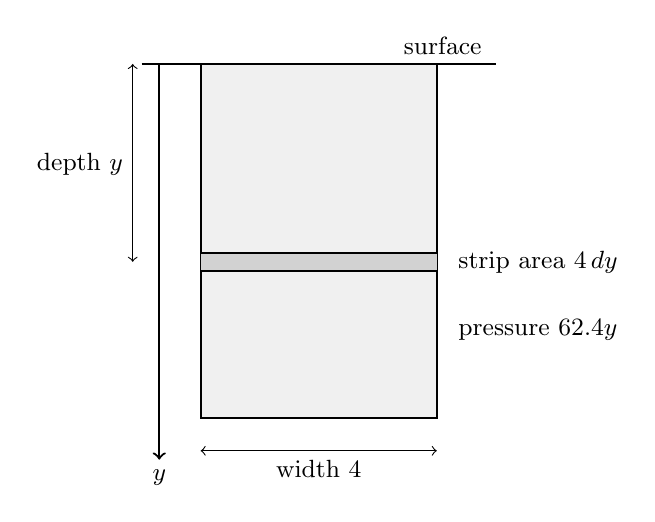
\begin{tikzpicture}[scale=0.75, every node/.style={font=\small}]
  % water surface
  \draw[thick] (-1,0) -- (5,0);
  \node[above] at (4.1,0) {surface};

  % plate
  \draw[thick, fill=gray!12] (0,-6) rectangle (4,0);

  % strip
  \fill[gray!35] (0,-3.5) rectangle (4,-3.2);
  \draw[thick] (0,-3.5) -- (4,-3.5);
  \draw[thick] (0,-3.2) -- (4,-3.2);

  % depth axis
  \draw[->, thick] (-0.7,0) -- (-0.7,-6.7);
  \node[below] at (-0.7,-6.7) {\(y\)};
  \draw[<->] (-1.15,0) -- (-1.15,-3.35);
  \node[left] at (-1.15,-1.7) {depth \(y\)};

  % width
  \draw[<->] (0,-6.55) -- (4,-6.55);
  \node[below] at (2,-6.55) {width \(4\)};

  % label
  \node[right] at (4.2,-3.35) {strip area \(4\,dy\)};
  \node[right] at (4.2,-4.5) {pressure \(62.4y\)};
\end{tikzpicture}
\caption{A horizontal strip has nearly constant pressure because its depth is nearly constant.}
\label{fig:hydrostatic-rectangular-plate}
\end{figure}

This example contains the general method.

At depth \(y\), suppose the horizontal width of the plate is \(w(y)\).  Then a thin strip
has area

\[
w(y)\,dy.
\]

The pressure is

\[
\gamma y.
\]

So the strip force is

\[
dF=\gamma y w(y)\,dy.
\]

\begin{quote}
\textbf{Hydrostatic force on a vertical plate.}
If \(y\) measures depth below the fluid surface, and the plate has horizontal width
\(w(y)\) at depth \(y\), then

\[
\boxed{
F=\gamma\int_a^b y\,w(y)\,dy.
}
\]

Here \(a\) and \(b\) are the smallest and largest depths of the plate.
\end{quote}

The formula is short, but the real work is choosing the coordinate and writing \(w(y)\).

\subsection{Choosing strips}
\label{subsec:choosing-strips-hydrostatic}

Hydrostatic pressure depends on depth.  So horizontal strips are natural.

A vertical strip would contain many depths at once, and the pressure would vary along
the strip.  A horizontal strip stays at one depth, up to a tiny error that disappears in the
limit.

\[
\boxed{
\text{For hydrostatic force on a vertical plate, use horizontal strips.}
}
\]

\paragraph{Example: a triangular plate, point down.}
A triangular plate has base \(4\) feet long at the water surface and vertex \(6\) feet
below the surface.  Find the force of the water on one side.

Let \(y\) be depth below the surface.

At \(y=0\), the width is \(4\).  At \(y=6\), the width is \(0\).  The width decreases
linearly, so

\[
w(y)=4\left(1-\frac{y}{6}\right).
\]

Thus

\[
F=62.4\int_0^6 y\cdot4\left(1-\frac{y}{6}\right)\,dy.
\]

Compute:

\[
F
=
249.6\int_0^6 \left(y-\frac{y^2}{6}\right)\,dy.
\]

Now

\[
\int_0^6 \left(y-\frac{y^2}{6}\right)\,dy
=
\left(\frac{y^2}{2}-\frac{y^3}{18}\right)\Big|_0^6.
\]

At \(y=6\),

\[
\frac{36}{2}-\frac{216}{18}
=
18-12
=
6.
\]

So

\[
F=249.6(6)=\boxed{1497.6}
\]

pounds.

\begin{figure}[h]
\centering
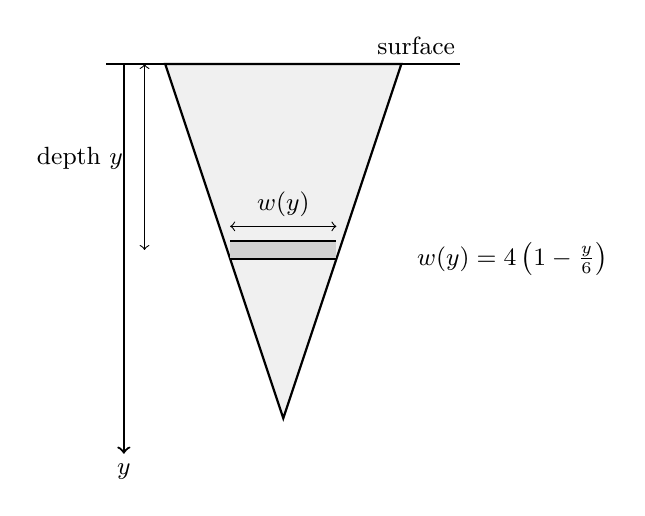
\begin{tikzpicture}[scale=0.75, every node/.style={font=\small}]
  % surface
  \draw[thick] (-3,0) -- (3,0);
  \node[above] at (2.25,0) {surface};

  % triangle
  \draw[thick, fill=gray!12] (-2,0) -- (2,0) -- (0,-6) -- cycle;

  % strip
  \fill[gray!35] (-0.9,-3.3) rectangle (0.9,-3.0);
  \draw[thick] (-0.9,-3.3) -- (0.9,-3.3);
  \draw[thick] (-0.9,-3.0) -- (0.9,-3.0);

  % depth marker
  \draw[->, thick] (-2.7,0) -- (-2.7,-6.6);
  \node[below] at (-2.7,-6.6) {\(y\)};
  \draw[<->] (-2.35,0) -- (-2.35,-3.15);
  \node[left] at (-2.55,-1.6) {depth \(y\)};

  % width
  \draw[<->] (-0.9,-2.75) -- (0.9,-2.75);
  \node[above] at (0,-2.75) {\(w(y)\)};

  \node[right] at (2.1,-3.3) {\(w(y)=4\left(1-\frac{y}{6}\right)\)};
\end{tikzpicture}
\caption{For the triangular plate, the strip width is a linear function of depth.}
\label{fig:hydrostatic-triangle}
\end{figure}

\paragraph{Same area, different force.}
Now turn the same triangular plate upside down: vertex at the surface, base \(4\) feet
long at depth \(6\) feet.

The area of the triangle is the same.  But more area is now deeper, where pressure is
larger.

The width at depth \(y\) is

\[
w(y)=\frac{4}{6}y=\frac{2}{3}y.
\]

So

\[
F=62.4\int_0^6 y\left(\frac23y\right)\,dy.
\]

Compute:

\[
F
=
62.4\cdot\frac23\int_0^6 y^2\,dy
=
62.4\cdot\frac23\left(\frac{y^3}{3}\right)\Big|_0^6.
\]

Thus

\[
F
=
62.4\cdot\frac23\cdot72
=
\boxed{2995.2}
\]

pounds.

This is twice the previous force.

\begin{quote}
\textbf{Warning.}
Hydrostatic force is not determined by area alone.  Depth matters.

Two plates with the same area can feel different total forces if one has more of its
area deeper in the water.
\end{quote}

\subsection{Dams and windows}
\label{subsec:dams-and-windows}

Dams and underwater windows are the most common places where hydrostatic force
matters.

A dam is wide, and the water depth changes from top to bottom.  A window may be
small, but the pressure can still be large if it is deep.

\paragraph{Example: a rectangular dam face.}
A vertical rectangular dam face is \(30\) meters wide.  The water is \(12\) meters deep.
Find the total force of the water on the dam face.

Use metric units.  For water,

\[
\gamma\approx9800\text{ N/m}^3.
\]

Let \(y\) be depth below the surface.  Then

\[
0\le y\le12.
\]

The width is constant:

\[
w(y)=30.
\]

So

\[
F=9800\int_0^{12} 30y\,dy.
\]

Compute:

\[
F=9800\cdot30\left(\frac{y^2}{2}\right)\Big|_0^{12}.
\]

Thus

\[
F=9800\cdot30\cdot72.
\]

Therefore

\[
\boxed{
F=21{,}168{,}000\text{ newtons}.
}
\]

The pressure at the bottom is large, but we did not multiply bottom pressure by the
whole area.  That would overestimate the force because the upper part has smaller
pressure.

\paragraph{A centroid shortcut.}
There is a useful shortcut for total force on a flat vertical plate.

The force is

\[
F=\gamma\int_D y\,dA,
\]

where \(D\) is the plate and \(y\) is depth below the surface.  If the plate has area \(A\)
and centroid depth \(\bar y\), then

\[
\int_D y\,dA=A\bar y.
\]

So

\[
\boxed{
F=\gamma A\bar y.
}
\]

This connects directly with moments from the last section.  The total hydrostatic force
is pressure at the centroid depth times area:

\[
F=(\gamma\bar y)A.
\]

This gives the total force.  It does not tell where the single equivalent force acts.  That
point is called the center of pressure, and it usually lies below the centroid.

\paragraph{Example: a circular underwater window.}
A circular window of radius \(1\) meter is vertical in the side of a tank.  Its center is
\(3\) meters below the water surface.  Find the total force on the window.

The area is

\[
A=\pi(1)^2=\pi.
\]

By symmetry, the centroid is the center of the circle, so

\[
\bar y=3.
\]

Using the centroid shortcut,

\[
F=\gamma A\bar y
=
9800(\pi)(3).
\]

Thus

\[
\boxed{
F=29{,}400\pi
}
\]

newtons.

We can also see the same result from strips.  At depth \(y\), the width of the circular
strip is

\[
2\sqrt{1-(y-3)^2},
\]

for

\[
2\le y\le4.
\]

So

\[
F=9800\int_2^4 y\,2\sqrt{1-(y-3)^2}\,dy.
\]

Let

\[
u=y-3.
\]

Then \(y=u+3\), and the limits become \(-1\) and \(1\).  The integral becomes

\[
9800\int_{-1}^1 (u+3)2\sqrt{1-u^2}\,du.
\]

Split it:

\[
9800\left[
\int_{-1}^1 2u\sqrt{1-u^2}\,du
+
3\int_{-1}^1 2\sqrt{1-u^2}\,du
\right].
\]

The first integrand is odd, so its integral over \([-1,1]\) is \(0\).  The second integral
is the area of a unit circle:

\[
\int_{-1}^1 2\sqrt{1-u^2}\,du=\pi.
\]

Therefore

\[
F=9800(3\pi)=29{,}400\pi,
\]

as before.

\begin{figure}[h]
\centering
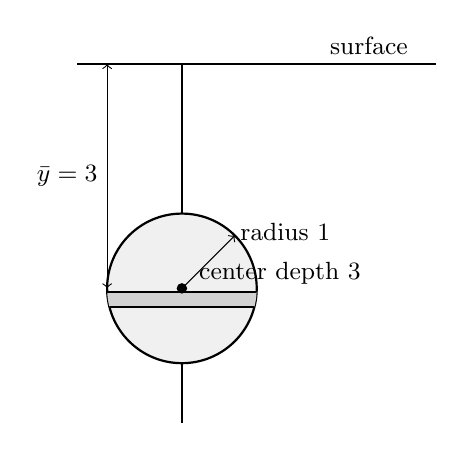
\begin{tikzpicture}[scale=0.95, every node/.style={font=\small}]
  % water surface
  \draw[thick] (-1.4,0) -- (3.4,0);
  \node[above] at (2.5,0) {surface};

  % tank wall
  \draw[thick] (0,0) -- (0,-4.8);

  % circular window
  \fill[gray!12] (0,-3) circle (1);
  \draw[thick] (0,-3) circle (1);

  % strip (clipped to perfectly match the circle boundary)
  \begin{scope}
    \clip (0,-3) circle (1);
    \fill[gray!35] (-1.5,-3.25) rectangle (1.5,-3.05);
    \draw[thick] (-1.5,-3.25) -- (1.5,-3.25);
    \draw[thick] (-1.5,-3.05) -- (1.5,-3.05);
  \end{scope}

  % center
  \fill (0,-3) circle (2pt);
  \node[right] at (0.1,-2.8) {center depth \(3\)};

  % depth arrow
  \draw[<->] (-1.0,0) -- (-1.0,-3);
  \node[left] at (-1.0,-1.5) {\(\bar y=3\)};

  % radius
  \draw[->] (0,-3) -- (0.707,-2.293);
  \node[right] at (0.65,-2.25) {radius \(1\)};
\end{tikzpicture}
\caption{For a symmetric vertical window, the centroid depth gives the total force quickly.}
\label{fig:hydrostatic-circular-window}
\end{figure}

\subsection{What hydrostatic force is measuring}
\label{subsec:what-hydrostatic-force-measures}

Hydrostatic force is another accumulation problem.

Area problems used

\[
dA=(\text{height})(dx).
\]

Volume problems used

\[
dV=(\text{cross-sectional area})(dx).
\]

Mass problems used

\[
dm=(\text{density})(\text{small length or area}).
\]

Work problems used

\[
dW=(\text{force})(\text{small displacement}).
\]

Hydrostatic force uses

\[
dF=(\text{pressure})(\text{small area}).
\]

Since pressure depends on depth,

\[
p=\gamma y,
\]

the strip at depth \(y\) contributes

\[
dF=\gamma y\,w(y)\,dy.
\]

The pattern has not changed:

\[
\boxed{
\text{find the small piece, write its contribution, and add.}
}
\]

We have now used integrals to measure area, volume, mass, center of mass, work, and
force.  One more common question remains:

\[
\text{What single number represents a varying quantity over an interval?}
\]

That question leads to average value.  From there, the same integral language will begin
to measure probability.
\section{Average value and probability}
\label{sec:average-value-probability}

Hydrostatic force added pressure over area:

\[
dF=(\text{pressure})(\text{small area}).
\]

Work added force over distance:

\[
dW=(\text{force})(\text{small displacement}).
\]

Mass added density over length or area.

Now we ask a quieter question.  Suppose a quantity changes over an interval.  What
single number best represents it?

If a car's velocity changes during a trip, we can still ask for its average velocity.  If a
temperature changes during a day, we can still ask for the average temperature.  If a
probability is spread over many possible outcomes, we can still ask for the expected
outcome.

The integral answers all of these by the same idea:

\[
\boxed{
\text{average}=\frac{\text{total accumulated amount}}{\text{size of the interval}}.
}
\]

\subsection{Average value of a continuous function}
\label{subsec:average-value-continuous-function}

Start with a familiar finite average.  If five test scores are

\[
82,\quad 90,\quad 76,\quad 88,\quad 94,
\]

then their average is

\[
\frac{82+90+76+88+94}{5}.
\]

We add the values and divide by the number of values.

For a function, there are infinitely many values on an interval.  We cannot add them one
by one.  But we can imitate the finite average with a Riemann sum.

Let \(f\) be continuous on \([a,b]\).  Divide the interval into \(n\) equal pieces.  Then

\[
\Delta x=\frac{b-a}{n}.
\]

Choose sample points

\[
x_1^*,x_2^*,\ldots,x_n^*
\]

in the subintervals.  The ordinary average of the sampled values is

\[
\frac{f(x_1^*)+f(x_2^*)+\cdots+f(x_n^*)}{n}.
\]

Since

\[
\frac1n=\frac{\Delta x}{b-a},
\]

this becomes

\[
\frac{1}{b-a}
\left(
f(x_1^*)\Delta x+f(x_2^*)\Delta x+\cdots+f(x_n^*)\Delta x
\right).
\]

As \(n\to\infty\), the sum inside the parentheses approaches

\[
\int_a^b f(x)\,dx.
\]

So the average value of \(f\) on \([a,b]\) is

\[
\boxed{
f_{\text{avg}}
=
\frac1{b-a}\int_a^b f(x)\,dx.
}
\]

This formula says:

\[
\boxed{
\int_a^b f(x)\,dx
=
(\text{average height})(\text{width}).
}
\]

So the average value is the height of a rectangle whose area matches the signed area
under the graph.

\paragraph{Example: average value of \(x^2\).}
Find the average value of

\[
f(x)=x^2
\]

on

\[
[0,3].
\]

By the formula,

\[
f_{\text{avg}}
=
\frac1{3-0}\int_0^3 x^2\,dx.
\]

Compute:

\[
f_{\text{avg}}
=
\frac13\left(\frac{x^3}{3}\right)\Big|_0^3
=
\frac13\cdot 9
=
\boxed{3}.
\]

So the average value of \(x^2\) on \([0,3]\) is \(3\).

This does not mean that \(x^2=3\) at the midpoint \(x=1.5\).  In fact,

\[
(1.5)^2=2.25.
\]

The average value is not usually the value at the midpoint.  It is the height that gives
the same accumulated area.

\begin{figure}[h]
\centering
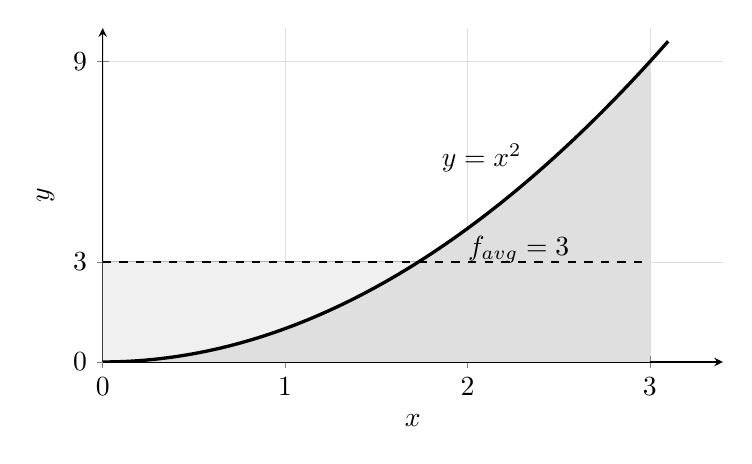
\begin{tikzpicture}
\begin{axis}[
    width=0.78\textwidth,
    height=0.48\textwidth,
    xmin=0, xmax=3.4,
    ymin=0, ymax=10,
    axis lines=left,
    xlabel={\(x\)},
    ylabel={\(y\)},
    xtick={0,1,2,3},
    ytick={0,3,9},
    grid=both,
    grid style={line width=.1pt, draw=gray!25},
]
% Rectangle of average height
\draw[fill=gray!12, draw=gray!60] (axis cs:0,0) rectangle (axis cs:3,3);

% Area under curve
\addplot[domain=0:3, samples=120, fill=gray!25, draw=none] {x^2} \closedcycle;

% Curve and average line
\addplot[very thick, domain=0:3.1, samples=120] {x^2};
\addplot[thick, dashed, domain=0:3, samples=2] {3};

\node[anchor=west] at (axis cs:1.95,3.35) {\(f_{\text{avg}}=3\)};
\node[anchor=east] at (axis cs:2.35,6.1) {\(y=x^2\)};
\end{axis}
\end{tikzpicture}
\caption{The average value is the height of a rectangle with the same area as the region under the graph.}
\label{fig:average-value-x-squared}
\end{figure}

\paragraph{Example: average velocity.}
If \(s(t)\) is position, then velocity is

\[
v(t)=s'(t).
\]

The average value of velocity on \([a,b]\) is

\[
v_{\text{avg}}
=
\frac1{b-a}\int_a^b v(t)\,dt.
\]

By the Fundamental Theorem,

\[
\int_a^b v(t)\,dt=s(b)-s(a).
\]

So

\[
v_{\text{avg}}
=
\frac{s(b)-s(a)}{b-a}.
\]

This is the average velocity we used at the beginning of the book.  The integral formula
has brought us back to the same idea:

\[
\boxed{
\text{average velocity}
=
\frac{\text{displacement}}{\text{elapsed time}}.
}
\]

\paragraph{Example: average temperature.}
Suppose the temperature during a \(12\)-hour period is modeled by

\[
T(t)=60+10\sin\left(\frac{\pi t}{12}\right),
\qquad 0\le t\le12,
\]

where \(t\) is measured in hours and \(T(t)\) in degrees Fahrenheit.

The average temperature is

\[
T_{\text{avg}}
=
\frac1{12}\int_0^{12}
\left(60+10\sin\left(\frac{\pi t}{12}\right)\right)\,dt.
\]

Compute the two parts:

\[
\frac1{12}\int_0^{12}60\,dt=60.
\]

For the sine part,

\[
\int_0^{12}10\sin\left(\frac{\pi t}{12}\right)\,dt
=
10\left[
-\frac{12}{\pi}\cos\left(\frac{\pi t}{12}\right)
\right]_0^{12}.
\]

Thus

\[
\int_0^{12}10\sin\left(\frac{\pi t}{12}\right)\,dt
=
-\frac{120}{\pi}\bigl(\cos\pi-\cos0\bigr).
\]

Since

\[
\cos\pi=-1,
\qquad
\cos0=1,
\]

we get

\[
-\frac{120}{\pi}(-2)=\frac{240}{\pi}.
\]

Therefore

\[
T_{\text{avg}}
=
60+\frac1{12}\cdot\frac{240}{\pi}
=
\boxed{
60+\frac{20}{\pi}
}.
\]

Numerically,

\[
T_{\text{avg}}\approx 66.37.
\]

The average is above \(60\) because this \(12\)-hour interval covers the positive half of
the sine wave.

\subsection{The average value theorem for integrals}
\label{subsec:average-value-theorem-integrals}

For \(f(x)=x^2\) on \([0,3]\), the average value was \(3\).  Since

\[
x^2=3
\]

when

\[
x=\sqrt3,
\]

the graph actually reaches its average height.

That is guaranteed for continuous functions.

\begin{quote}
\textbf{Average value theorem for integrals.}
If \(f\) is continuous on \([a,b]\), then there is at least one number \(c\in[a,b]\) such
that

\[
\boxed{
f(c)=\frac1{b-a}\int_a^b f(x)\,dx.
}
\]
\end{quote}

In words:

\[
\boxed{
\text{A continuous function reaches its average value somewhere.}
}
\]

\paragraph{Idea of the proof.}
Because \(f\) is continuous on \([a,b]\), the Extreme Value Theorem says that \(f\)
has an absolute minimum \(m\) and an absolute maximum \(M\) on the interval.

So

\[
m\le f(x)\le M
\]

for every \(x\in[a,b]\).  Integrating gives

\[
m(b-a)\le \int_a^b f(x)\,dx\le M(b-a).
\]

Divide by \(b-a>0\):

\[
m\le
\frac1{b-a}\int_a^b f(x)\,dx
\le M.
\]

Thus the average value lies between the minimum and the maximum.  Since \(f\) is
continuous, the Intermediate Value Theorem says that \(f\) takes every value between
\(m\) and \(M\).  Therefore \(f\) takes its average value at some point \(c\).

\paragraph{Why continuity matters.}
The average value can exist even when the function is not continuous.  But without
continuity, the function may not actually equal its average anywhere.

Define

\[
f(x)=
\begin{cases}
0, & 0\le x<\frac12,\\
1, & \frac12\le x\le1.
\end{cases}
\]

Then

\[
\int_0^1 f(x)\,dx=\frac12.
\]

So the average value is

\[
f_{\text{avg}}
=
\frac1{1-0}\int_0^1 f(x)\,dx
=
\frac12.
\]

But \(f(x)\) is only \(0\) or \(1\).  It is never equal to \(\frac12\).

\begin{quote}
\textbf{Moral.}
The formula

\[
f_{\text{avg}}=\frac1{b-a}\int_a^b f(x)\,dx
\]

can make sense for many integrable functions.  But the guarantee that the function
actually reaches its average value uses continuity.
\end{quote}

\subsection{Probability density}
\label{subsec:probability-density}

Area can also measure probability.

Imagine a spinner that can land anywhere between \(0\) and \(1\).  If all positions are
equally likely, then the probability of landing between \(0.2\) and \(0.5\) should be the
length of that interval:

\[
0.5-0.2=0.3.
\]

Here probability is spread uniformly over \([0,1]\).  The density is

\[
p(x)=1.
\]

Then

\[
P(0.2\le X\le0.5)
=
\int_{0.2}^{0.5}1\,dx
=
0.3.
\]

The integral has become probability.

\begin{quote}
\textbf{Probability density on an interval.}
A function \(p(x)\) is a probability density on \([a,b]\) if

\[
p(x)\ge0
\]

and

\[
\boxed{
\int_a^b p(x)\,dx=1.
}
\]

Then the probability that the outcome \(X\) lies between \(c\) and \(d\), where
\(a\le c\le d\le b\), is

\[
\boxed{
P(c\le X\le d)=\int_c^d p(x)\,dx.
}
\]
\end{quote}

The total area under a probability density is \(1\), because total probability is \(1\).

\paragraph{Example: a triangular density.}
Let

\[
p(x)=2x,
\qquad 0\le x\le1.
\]

First check that this is a density:

\[
\int_0^1 2x\,dx
=
x^2\Big|_0^1
=
1.
\]

Also,

\[
p(x)\ge0
\]

on \([0,1]\).  So \(p\) is a probability density.

Now find

\[
P\left(0\le X\le\frac12\right).
\]

We compute

\[
P\left(0\le X\le\frac12\right)
=
\int_0^{1/2}2x\,dx
=
x^2\Big|_0^{1/2}
=
\frac14.
\]

So the probability that \(X\) lies in the left half of the interval is only

\[
\boxed{\frac14}.
\]

The right half has probability

\[
1-\frac14=\frac34.
\]

That makes sense because the density \(p(x)=2x\) is larger near \(1\) than near \(0\).

\begin{figure}[h]
\centering
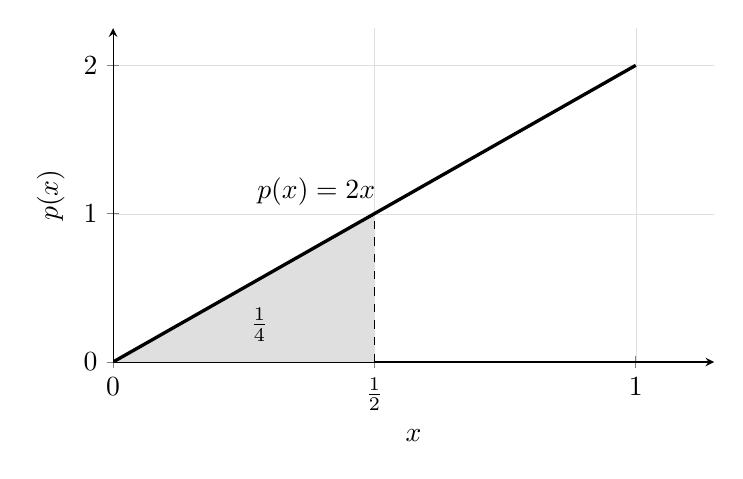
\begin{tikzpicture}
\begin{axis}[
    width=0.76\textwidth,
    height=0.48\textwidth,
    xmin=0, xmax=1.15,
    ymin=0, ymax=2.25,
    axis lines=left,
    xlabel={\(x\)},
    ylabel={\(p(x)\)},
    xtick={0,0.5,1},
    xticklabels={\(0\),\(\frac12\),\(1\)},
    ytick={0,1,2},
    grid=both,
    grid style={line width=.1pt, draw=gray!25},
]
\addplot[domain=0:0.5, samples=2, fill=gray!25, draw=none] {2*x} \closedcycle;
\addplot[very thick, domain=0:1, samples=2] {2*x};
\draw[dashed] (axis cs:0.5,0) -- (axis cs:0.5,1);
\node[anchor=east] at (axis cs:0.52,1.15) {\(p(x)=2x\)};
\node at (axis cs:0.28,0.25) {\(\frac14\)};
\end{axis}
\end{tikzpicture}
\caption{For the density \(p(x)=2x\), probability is area under the density curve.}
\label{fig:triangular-density}
\end{figure}

\paragraph{Density is not probability.}
A probability is between \(0\) and \(1\).  A density does not have to be.

For example, define

\[
p(x)=4,
\qquad 0\le x\le\frac14.
\]

Then

\[
\int_0^{1/4}4\,dx=1,
\]

so this is a probability density on \([0,\frac14]\).  The density value \(4\) is bigger
than \(1\), and that is not a problem.

The probability of an interval is area:

\[
P\left(0\le X\le \frac{1}{10}\right)
=
\int_0^{1/10}4\,dx
=
\frac{4}{10}
=
0.4.
\]

\begin{quote}
\textbf{Warning.}
A density value is not a probability.  A density measures probability per unit length.
Only an integral of density over an interval gives probability.
\end{quote}

\subsection{Expected value}
\label{subsec:expected-value}

Average value and probability meet in the idea of expected value.

For a finite list of outcomes, a weighted average has the form

\[
(\text{outcome})(\text{weight})
+
(\text{outcome})(\text{weight})
+
\cdots.
\]

For a continuous density, the small probability near \(x\) is approximately

\[
p(x)\,dx.
\]

So the small contribution to the average outcome is

\[
x\,p(x)\,dx.
\]

Adding gives the expected value.

\begin{quote}
\textbf{Expected value.}
If \(X\) has probability density \(p(x)\) on \([a,b]\), then its expected value is

\[
\boxed{
E[X]=\int_a^b x\,p(x)\,dx.
}
\]
\end{quote}

The expected value is the balance point of the probability distribution.  It is the
probability version of center of mass.

\paragraph{Example: expected value of a uniform density.}
Let

\[
p(x)=\frac1{b-a},
\qquad a\le x\le b.
\]

This is uniform density on \([a,b]\).  Then

\[
E[X]=\int_a^b x\frac1{b-a}\,dx.
\]

Compute:

\[
E[X]
=
\frac1{b-a}\left(\frac{x^2}{2}\right)\Big|_a^b
=
\frac{b^2-a^2}{2(b-a)}.
\]

Factor:

\[
b^2-a^2=(b-a)(b+a).
\]

So

\[
E[X]
=
\boxed{
\frac{a+b}{2}
}.
\]

A uniform distribution balances at the midpoint.

\paragraph{Example: expected value for the triangular density.}
For

\[
p(x)=2x,
\qquad 0\le x\le1,
\]

the expected value is

\[
E[X]=\int_0^1 x(2x)\,dx.
\]

Thus

\[
E[X]=\int_0^1 2x^2\,dx
=
\frac{2x^3}{3}\Big|_0^1
=
\boxed{\frac23}.
\]

The expected value is to the right of the midpoint \(\frac12\), because the density is
heavier near \(1\).

\begin{quote}
\textbf{Center of mass analogy.}
For a rod with density \(\lambda(x)\),

\[
\bar x=\frac{\int x\lambda(x)\,dx}{\int \lambda(x)\,dx}.
\]

For a probability density \(p(x)\),

\[
E[X]=\int x p(x)\,dx,
\]

because

\[
\int p(x)\,dx=1.
\]

Probability density is mass density with total mass normalized to \(1\).
\end{quote}

\subsection{Normal distribution as a preview of non-elementary integrals}
\label{subsec:normal-distribution-preview}

Many real measurements cluster around a typical value: measurement errors, biological
variation, repeated experimental noise.  A common model is the normal distribution.

The normal density with mean \(\mu\) and standard deviation \(\sigma\) is

\[
p(x)
=
\frac{1}{\sigma\sqrt{2\pi}}
e^{-\frac{(x-\mu)^2}{2\sigma^2}}.
\]

The parameter \(\mu\) gives the center.  The parameter \(\sigma\) controls the spread.

The standard normal density has

\[
\mu=0,
\qquad
\sigma=1.
\]

It is

\[
\phi(x)=\frac1{\sqrt{2\pi}}e^{-x^2/2}.
\]

\begin{figure}[h]
\centering
\begin{tikzpicture}
\begin{axis}[
    width=0.78\textwidth,
    height=0.48\textwidth,
    xmin=-4, xmax=4,
    ymin=0, ymax=0.45,
    axis lines=left,
    xlabel={\(x\)},
    ylabel={\(\phi(x)\)},
    xtick={-3,-2,-1,0,1,2,3},
    ytick={0,0.2,0.4},
    grid=both,
    grid style={line width=.1pt, draw=gray!25},
]
\addplot[domain=-1:1, samples=120, fill=gray!25, draw=none]
    {exp(-x^2/2)/sqrt(2*pi)} \closedcycle;
\addplot[very thick, domain=-4:4, samples=250]
    {exp(-x^2/2)/sqrt(2*pi)};
\draw[dashed] (axis cs:-1,0) -- (axis cs:-1,0.242);
\draw[dashed] (axis cs:1,0) -- (axis cs:1,0.242);
\node[anchor=west] at (axis cs:1.15,0.30) {\(\phi(x)=\dfrac1{\sqrt{2\pi}}e^{-x^2/2}\)};
\node at (axis cs:0,0.08) {area \(=P(-1\le X\le1)\)};
\end{axis}
\end{tikzpicture}
\caption{For a normal density, probabilities are areas under the bell-shaped curve.}
\label{fig:standard-normal-density}
\end{figure}

If \(X\) has standard normal density, then

\[
P(-1\le X\le1)
=
\int_{-1}^{1}
\frac1{\sqrt{2\pi}}e^{-x^2/2}\,dx.
\]

This integral has a perfectly clear meaning: it is an area, and therefore a probability.

But there is a surprise.  The function

\[
e^{-x^2/2}
\]

does not have an elementary antiderivative.  That means no combination of the usual
functions from algebra, trigonometry, exponentials, and logarithms gives an exact
antiderivative.

So probability leads naturally to integrals that are meaningful but not elementary.

For the standard normal distribution, we define the accumulation function

\[
\Phi(z)=\int_{-\infty}^{z}
\frac1{\sqrt{2\pi}}e^{-x^2/2}\,dx.
\]

The infinite endpoint will be made precise later when we study improper integrals.
For now, the meaning is this: \(\Phi(z)\) is the probability that a standard normal
variable is at most \(z\).

\[
\boxed{
\Phi(z)=P(X\le z).
}
\]

The values of \(\Phi\) are found by numerical integration, tables, or technology.

\begin{quote}
\textbf{What probability teaches us.}
A definite integral may have an exact meaning even when no elementary antiderivative
exists.  The integral can define a new function.
\end{quote}

Average value and probability both use integrals to summarize spread-out information.
The next section changes the geometry again.  Instead of adding vertical strips, slices,
or forces, we add tiny pieces of a curve itself.

\section{Arc length and surface area of revolution}
\label{sec:arc-length-surface-area-revolution}

Area comes from small rectangles.  Volume comes from small slices.  Work comes from
small force-times-distance pieces.

Length should come from small straight pieces.

A curve is not straight, but if we zoom in far enough, a smooth curve looks almost like
a line segment.  So the small piece of length is not just \(dx\).  It is a slanted distance:

\[
ds\approx \sqrt{(dx)^2+(dy)^2}.
\]

That is the new small piece.

\subsection{Arc length from small straight pieces}
\label{subsec:arc-length-small-straight-pieces}

Suppose a curve is the graph of

\[
y=f(x),
\qquad a\le x\le b.
\]

Divide the interval \([a,b]\) into small pieces:

\[
a=x_0<x_1<\cdots<x_n=b.
\]

The corresponding points on the graph are

\[
(x_0,f(x_0)),\quad (x_1,f(x_1)),\quad \ldots,\quad (x_n,f(x_n)).
\]

Join these points by straight line segments.  The polygonal path approximates the curve.

The length of the segment from \(x_{i-1}\) to \(x_i\) is

\[
\sqrt{(x_i-x_{i-1})^2+\bigl(f(x_i)-f(x_{i-1})\bigr)^2}.
\]

Write

\[
\Delta x_i=x_i-x_{i-1}
\]

and

\[
\Delta y_i=f(x_i)-f(x_{i-1}).
\]

Then the small segment length is

\[
\sqrt{(\Delta x_i)^2+(\Delta y_i)^2}.
\]

Factor out \(\Delta x_i\):

\[
\sqrt{(\Delta x_i)^2+(\Delta y_i)^2}
=
\sqrt{1+\left(\frac{\Delta y_i}{\Delta x_i}\right)^2}\,\Delta x_i.
\]

When the pieces are small,

\[
\frac{\Delta y_i}{\Delta x_i}
\]

is close to a derivative value.  Thus the small length is approximately

\[
\sqrt{1+\bigl(f'(x)\bigr)^2}\,dx.
\]

So

\[
\boxed{
ds=\sqrt{1+\bigl(f'(x)\bigr)^2}\,dx.
}
\]

\begin{figure}[h]
\centering
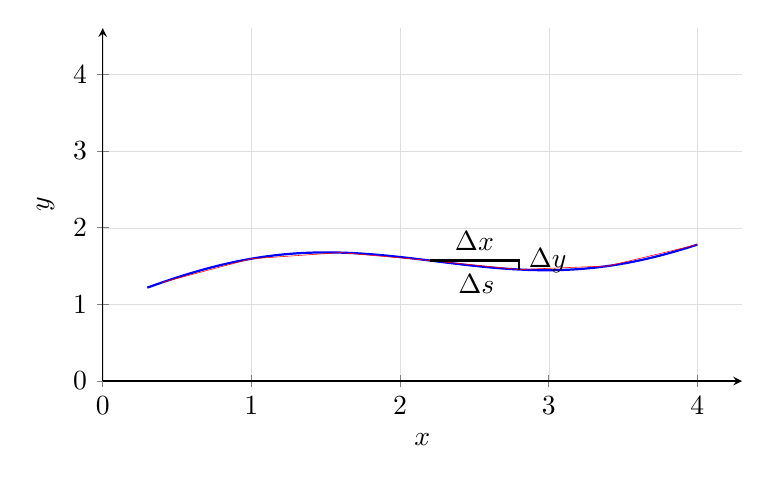
\begin{tikzpicture}
\begin{axis}[
    width=0.80\textwidth,
    height=0.50\textwidth,
    xmin=0, xmax=4.3,
    ymin=0, ymax=4.6,
    axis lines=left,
    xlabel={\(x\)},
    ylabel={\(y\)},
    xtick={0,1,2,3,4},
    ytick={0,1,2,3,4},
    grid=both,
    grid style={line width=.1pt, draw=gray!25},
]
\addplot[blue, thick, domain=0.3:4, samples=200] {1+0.25*x+0.35*sin(deg(1.4*x))};

% polygonal approximation (samples=7 automatically computes your 7 spaced coordinates)
\addplot[red, very thin, mark=none, domain=0.4:4.0, samples=7] {1+0.25*x+0.35*sin(deg(1.4*x))};

% evaluated heights at x=2.2 and x=2.8 for cleaner drawing
\draw[thick] (axis cs:2.2, 1.572) -- (axis cs:2.8, 1.572) -- (axis cs:2.8, 1.453);

% anchored directly to the midpoints of the triangle legs
\node[anchor=south]      at (axis cs:2.5, 1.572) {\(\Delta x\)};
\node[anchor=west]       at (axis cs:2.8, 1.57) {\(\Delta y\)};
\node[anchor=north east] at (axis cs:2.7, 1.513) {\(\Delta s\)};
\end{axis}
\end{tikzpicture}
\caption{A smooth curve is approximated by short straight pieces.  Each small length comes from the Pythagorean theorem.}
\label{fig:arc-length-polygonal}
\end{figure}

\subsection{Arc length of a graph}
\label{subsec:arc-length-graph}

The limiting sum gives the arc length formula.

\begin{quote}
\textbf{Arc length of a graph.}
If \(f'\) is continuous on \([a,b]\), then the length of the graph

\[
y=f(x),
\qquad a\le x\le b,
\]

is

\[
\boxed{
L=\int_a^b \sqrt{1+\bigl(f'(x)\bigr)^2}\,dx.
}
\]
\end{quote}

In words:

\[
\boxed{
\text{length}=\int ds.
}
\]

Here

\[
ds=\sqrt{1+\bigl(f'(x)\bigr)^2}\,dx
\]

is the small slanted length along the curve.

\paragraph{Example: a line segment.}
Find the length of the graph

\[
y=mx+c
\]

from \(x=a\) to \(x=b\).

Since

\[
f'(x)=m,
\]

the arc length is

\[
L=\int_a^b \sqrt{1+m^2}\,dx.
\]

The integrand is constant, so

\[
L=\sqrt{1+m^2}(b-a).
\]

This agrees with the distance formula.  The endpoints are

\[
(a,ma+c)
\]

and

\[
(b,mb+c).
\]

The horizontal change is

\[
b-a,
\]

and the vertical change is

\[
m(b-a).
\]

So the distance is

\[
\sqrt{(b-a)^2+\bigl(m(b-a)\bigr)^2}
=
\sqrt{1+m^2}(b-a).
\]

The integral formula passes the first test.

\paragraph{Example: a curve chosen to make the length simple.}
Find the length of

\[
y=\frac23 x^{3/2}
\]

from \(x=0\) to \(x=3\).

First compute the derivative:

\[
y'=\frac23\cdot\frac32 x^{1/2}=\sqrt{x}.
\]

So

\[
1+(y')^2=1+x.
\]

The length is

\[
L=\int_0^3 \sqrt{1+x}\,dx.
\]

Let

\[
u=1+x.
\]

Then

\[
du=dx.
\]

When \(x=0\), \(u=1\).  When \(x=3\), \(u=4\).  Therefore

\[
L=\int_1^4 \sqrt{u}\,du.
\]

Compute:

\[
L=\left(\frac23u^{3/2}\right)\Big|_1^4
=
\frac23\left(4^{3/2}-1^{3/2}\right).
\]

Since

\[
4^{3/2}=8,
\]

we get

\[
L=\frac23(8-1)=\boxed{\frac{14}{3}}.
\]

\paragraph{Why not just integrate \(|f'(x)|\)?}
The integral

\[
\int_a^b |f'(x)|\,dx
\]

measures total vertical change, not length along the curve.

For the line

\[
y=x
\]

from \(x=0\) to \(x=1\),

\[
\int_0^1 |f'(x)|\,dx
=
\int_0^1 1\,dx
=
1.
\]

But the actual length of the line segment from \((0,0)\) to \((1,1)\) is

\[
\sqrt{1^2+1^2}=\sqrt2.
\]

The missing horizontal motion matters.

\begin{quote}
\textbf{Warning.}
Arc length uses

\[
ds=\sqrt{(dx)^2+(dy)^2},
\]

not only \(dy\).  A curve moves horizontally and vertically at the same time.
\end{quote}

\subsection{Surface area by rotating a curve}
\label{subsec:surface-area-rotating-curve}

A curve rotated around an axis sweeps out a surface.

For example, rotating a line segment around the \(x\)-axis can form the side of a cone.
Rotating a semicircle around the \(x\)-axis forms a sphere.

To find surface area, we again look at a small piece.

Suppose a small arc segment has length

\[
ds.
\]

If it is at height \(y\) above the \(x\)-axis and rotates around the \(x\)-axis, it sweeps
out a thin band.  The band is almost a rectangle when unwrapped.  Its width is

\[
ds,
\]

and its other dimension is the circumference

\[
2\pi y.
\]

So its area is approximately

\[
dS=2\pi y\,ds.
\]

For a graph \(y=f(x)\),

\[
ds=\sqrt{1+\bigl(f'(x)\bigr)^2}\,dx.
\]

Thus

\[
dS
=
2\pi f(x)\sqrt{1+\bigl(f'(x)\bigr)^2}\,dx.
\]

\begin{quote}
\textbf{Surface area around the \(x\)-axis.}
If \(f(x)\ge0\) and \(f'\) is continuous on \([a,b]\), then the surface area formed by
rotating

\[
y=f(x),
\qquad a\le x\le b,
\]

around the \(x\)-axis is

\[
\boxed{
S=2\pi\int_a^b f(x)\sqrt{1+\bigl(f'(x)\bigr)^2}\,dx.
}
\]
\end{quote}

In words:

\[
\boxed{
\text{surface area}
=
\int(\text{circumference})(\text{small arc length}).
}
\]

The formula is the surface-area cousin of the shell method:

\[
\text{circumference}\cdot\text{height}\cdot\text{thickness}.
\]

Here the ``height'' of the unwrapped band is the small arc length \(ds\).

\begin{figure}[h]
\centering
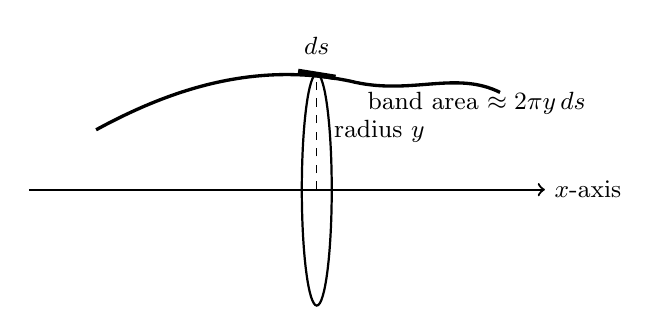
\begin{tikzpicture}[scale=0.95, every node/.style={font=\small}]
  % axis
  \draw[->, thick] (-0.3,0) -- (6.6,0);
  \node[right] at (6.6,0) {\(x\)-axis};

  % curve
  \draw[very thick]
    (0.6,0.8)
    .. controls (1.7,1.4) and (2.8,1.7) .. (4.0,1.45)
    .. controls (4.8,1.25) and (5.4,1.6) .. (6.0,1.3);

  % small segment
  \draw[line width=2pt] (3.3,1.58) -- (3.8,1.50);
  \node[above] at (3.55,1.68) {\(ds\)};

  % rotation ellipse
  \draw[thick] (3.55,0) ellipse (0.20 and 1.55);
  \draw[dashed] (3.55,0) -- (3.55,1.55);
  \node[right] at (3.65,0.78) {radius \(y\)};
  \node[right] at (4.1,1.15) {band area \(\approx 2\pi y\,ds\)};
\end{tikzpicture}
\caption{A small arc segment rotated around the \(x\)-axis sweeps out a thin band.}
\label{fig:surface-area-band}
\end{figure}

If the graph is rotated around the \(y\)-axis instead, the radius is \(x\), assuming
\(x\ge0\).  Then

\[
\boxed{
S=2\pi\int_a^b x\sqrt{1+\bigl(f'(x)\bigr)^2}\,dx.
}
\]

More generally, the radius is always the distance to the axis of rotation.

\subsection{Cone surface area from the integral}
\label{subsec:cone-surface-area-integral}

A right circular cone has height \(h\) and base radius \(R\).  We can get its side surface
by rotating the line segment

\[
y=\frac{R}{h}x,
\qquad 0\le x\le h,
\]

around the \(x\)-axis.

This produces only the curved side surface, not the circular base.

Here

\[
f(x)=\frac{R}{h}x,
\]

so

\[
f'(x)=\frac{R}{h}.
\]

Thus

\[
\sqrt{1+\bigl(f'(x)\bigr)^2}
=
\sqrt{1+\frac{R^2}{h^2}}
=
\frac{\sqrt{h^2+R^2}}{h}.
\]

The surface area is

\[
S
=
2\pi\int_0^h
\frac{R}{h}x
\cdot
\frac{\sqrt{h^2+R^2}}{h}
\,dx.
\]

Factor out constants:

\[
S
=
\frac{2\pi R\sqrt{h^2+R^2}}{h^2}
\int_0^h x\,dx.
\]

Compute:

\[
\int_0^h x\,dx=\frac{h^2}{2}.
\]

Therefore

\[
S
=
\frac{2\pi R\sqrt{h^2+R^2}}{h^2}\cdot\frac{h^2}{2}.
\]

So

\[
\boxed{
S=\pi R\sqrt{h^2+R^2}.
}
\]

The quantity

\[
\sqrt{h^2+R^2}
\]

is the slant height of the cone.  So this agrees with the familiar formula

\[
S=\pi R(\text{slant height}).
\]

\begin{quote}
\textbf{What the integral added.}
The formula for a cone's side area is not a separate fact to memorize.  It comes from
adding the circumferences of tiny slanted bands.
\end{quote}

\subsection{Sphere surface area from the integral}
\label{subsec:sphere-surface-area-integral}

The upper semicircle

\[
y=\sqrt{R^2-x^2},
\qquad -R\le x\le R,
\]

rotated around the \(x\)-axis forms a sphere of radius \(R\).

For \(-R<x<R\),

\[
y'=\frac{-x}{\sqrt{R^2-x^2}}.
\]

Then

\[
1+(y')^2
=
1+\frac{x^2}{R^2-x^2}
=
\frac{R^2}{R^2-x^2}.
\]

So

\[
\sqrt{1+(y')^2}
=
\frac{R}{\sqrt{R^2-x^2}}.
\]

Now multiply by \(y\):

\[
y\sqrt{1+(y')^2}
=
\sqrt{R^2-x^2}\cdot
\frac{R}{\sqrt{R^2-x^2}}
=
R.
\]

The surface area is therefore

\[
S
=
2\pi\int_{-R}^{R} R\,dx.
\]

So

\[
S
=
2\pi R(2R)
=
\boxed{4\pi R^2}.
\]

The derivative of the semicircle becomes infinite at the endpoints, but the surface-area
integrand simplifies to the constant \(2\pi R\).  The limiting surface area is finite.

\begin{figure}[h]
\centering
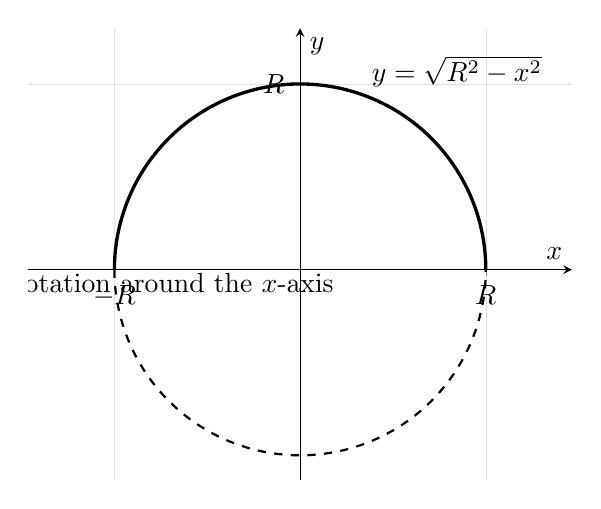
\begin{tikzpicture}
\begin{axis}[
    width=0.70\textwidth,
    axis equal,
    xmin=-3.4, xmax=3.4,
    ymin=-3.4, ymax=3.9,
    axis lines=middle,
    xlabel={\(x\)},
    ylabel={\(y\)},
    xtick={-3,0,3},
    xticklabels={\(-R\),\(0\),\(R\)},
    ytick={0,3},
    yticklabels={\(0\),\(R\)},
    grid=both,
    grid style={line width=.1pt, draw=gray!25},
]
% Parametric plotting avoids endpoint evaluation gaps
\addplot[very thick, domain=0:180, samples=100, variable=\t] ({3*cos(\t)}, {3*sin(\t)});
\addplot[thick, dashed, domain=180:360, samples=100, variable=\t] ({3*cos(\t)}, {3*sin(\t)});

\node[anchor=west] at (axis cs:1.0,3.2) {\(y=\sqrt{R^2-x^2}\)};
\node[anchor=east] at (axis cs:0.7,-0.22) {rotation around the \(x\)-axis};
\end{axis}
\end{tikzpicture}
\caption{Rotating the upper semicircle around the \(x\)-axis produces a sphere.}
\label{fig:sphere-from-semicircle}
\end{figure}

The result

\[
4\pi R^2
\]

looks simple.  The cancellation in the integral explains why it is simple.

\subsection{Why some natural lengths have no elementary antiderivative}
\label{subsec:natural-lengths-no-elementary-antiderivative}

The arc length formula is powerful, but it often produces integrals that are hard to
evaluate.

For example, the length of

\[
y=\sin x
\]

from \(x=0\) to \(x=\pi\) is

\[
L=\int_0^\pi \sqrt{1+\cos^2 x}\,dx.
\]

This integral is meaningful.  It is the length of a familiar curve.

But

\[
\sqrt{1+\cos^2 x}
\]

has no elementary antiderivative.  So the exact length cannot be written using only the
usual elementary functions.  A numerical method gives

\[
L\approx 3.8202.
\]

\begin{figure}[h]
\centering
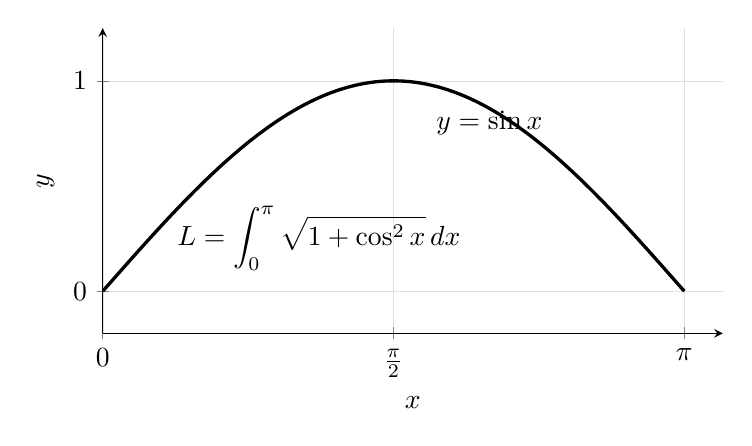
\begin{tikzpicture}
\begin{axis}[
    width=0.78\textwidth,
    height=0.45\textwidth,
    xmin=0, xmax=3.35,
    ymin=-0.2, ymax=1.25,
    axis lines=left,
    xlabel={\(x\)},
    ylabel={\(y\)},
    xtick={0,1.5708,3.1416},
    xticklabels={\(0\),\(\frac{\pi}{2}\),\(\pi\)},
    ytick={0,1},
    grid=both,
    grid style={line width=.1pt, draw=gray!25},
]
\addplot[very thick, domain=0:pi, samples=200] {sin(deg(x))};
\node[anchor=west] at (axis cs:1.75,0.8) {\(y=\sin x\)};
\node[anchor=west] at (axis cs:0.35,0.25) {\(L=\displaystyle\int_0^\pi \sqrt{1+\cos^2 x}\,dx\)};
\end{axis}
\end{tikzpicture}
\caption{Even a simple curve can lead to a length integral with no elementary antiderivative.}
\label{fig:sine-arc-length}
\end{figure}

This is an important moment in the story.

Setting up an integral and evaluating an integral are different skills.

The setup comes from meaning:

\[
\text{What is the small piece?}
\]

The evaluation comes from technique:

\[
\text{Can we find an antiderivative, or must we approximate?}
\]

Many applications produce correct, useful integrals that cannot be evaluated by the
methods we know so far.

\begin{quote}
\textbf{The lesson of arc length.}
The integral is not merely an antiderivative problem.  It is a way to define and measure
quantities.  Some of those quantities require new functions or numerical approximation.
\end{quote}

This chapter has asked what integrals measure.  We have measured area, volume, mass,
center of mass, work, hydrostatic force, average value, probability, length, and surface
area.

The next question is computational.

When the correct setup gives an integral such as

\[
\int x e^x\,dx,
\qquad
\int \sin^3 x\,dx,
\qquad
\int \sqrt{a^2-x^2}\,dx,
\]

we need more than the basic antiderivative rules.  The next chapter develops techniques
for finding antiderivatives when substitution alone is not enough.
\section{Chapter review and applications}
\label{sec:chapter10-review-applications}

This chapter has changed the shape of the small piece again and again.

At first the small piece was a strip of area:

\[
dA=(\text{height})\,dx.
\]

Then it became a slice of volume:

\[
dV=(\text{cross-sectional area})\,dx.
\]

Then it became a shell, a mass element, a moment, a work element, a pressure-force
element, a probability element, and a tiny slanted piece of length.

The question stayed the same:

\[
\boxed{
\text{What is one small piece, and what does it contribute?}
}
\]

That is the main skill of applications of integration.

\subsection{The chapter in one table}
\label{subsec:chapter10-small-piece-table}

The formulas in this chapter are easier to remember when they are organized by the
small piece they add.

\begin{center}
\renewcommand{\arraystretch}{1.45}
\begin{tabular}{p{0.22\textwidth}|p{0.34\textwidth}|p{0.35\textwidth}}
\textbf{quantity} & \textbf{small piece} & \textbf{typical integral} \\ \hline

area between curves &
\(\displaystyle dA=(\text{top}-\text{bottom})\,dx\) or
\(\displaystyle dA=(\text{right}-\text{left})\,dy\) &
\(\displaystyle A=\int_a^b (g(x)-f(x))\,dx\) \\

volume by slicing &
\(\displaystyle dV=A(x)\,dx\) &
\(\displaystyle V=\int_a^b A(x)\,dx\) \\

disk or washer volume &
\(\displaystyle dV=\pi\bigl(R(x)^2-r(x)^2\bigr)\,dx\) &
\(\displaystyle V=\pi\int_a^b \bigl(R(x)^2-r(x)^2\bigr)\,dx\) \\

shell volume &
\(\displaystyle dV=2\pi(\text{radius})(\text{height})(\text{thickness})\) &
\(\displaystyle V=2\pi\int_a^b xH(x)\,dx\) for shells about the \(y\)-axis \\

mass of a rod &
\(\displaystyle dm=\lambda(x)\,dx\) &
\(\displaystyle m=\int_a^b \lambda(x)\,dx\) \\

moment about the origin &
\(\displaystyle dM_0=x\,dm\) &
\(\displaystyle M_0=\int_a^b x\lambda(x)\,dx\) \\

work by a force &
\(\displaystyle dW=F(x)\,dx\) &
\(\displaystyle W=\int_a^b F(x)\,dx\) \\

work pumping fluid &
\(\displaystyle dW=\gamma A(y)D(y)\,dy\) &
\(\displaystyle W=\int \gamma A(y)D(y)\,dy\) \\

hydrostatic force &
\(\displaystyle dF=(\text{pressure})(\text{strip area})\) &
\(\displaystyle F=\gamma\int_a^b y\,w(y)\,dy\), when \(y\) is depth \\

probability &
\(\displaystyle dP=p(x)\,dx\) &
\(\displaystyle P(c\le X\le d)=\int_c^d p(x)\,dx\) \\

expected value &
\(\displaystyle dE=x\,dP=xp(x)\,dx\) &
\(\displaystyle E[X]=\int_a^b xp(x)\,dx\) \\

arc length &
\(\displaystyle ds=\sqrt{1+\bigl(f'(x)\bigr)^2}\,dx\) &
\(\displaystyle L=\int_a^b \sqrt{1+\bigl(f'(x)\bigr)^2}\,dx\) \\

surface area of revolution &
\(\displaystyle dS=2\pi(\text{radius})\,ds\) &
\(\displaystyle S=2\pi\int_a^b f(x)\sqrt{1+\bigl(f'(x)\bigr)^2}\,dx\)
\end{tabular}
\end{center}

The table is not meant to be memorized as a pile of formulas.  It is meant to show one
pattern:

\[
\boxed{
\text{integral}=\int(\text{contribution of one small piece}).
}
\]

\subsection{Skills: choose the small piece}
\label{subsec:skills-choose-small-piece}

The hardest step is usually not the antiderivative.  The hardest step is choosing what to
add.

A useful setup routine is:

\begin{quote}
\textbf{Application setup routine.}

\begin{enumerate}
\item Decide what quantity is being measured: area, volume, mass, work, force,
probability, length, or surface area.
\item Choose a slicing variable: usually \(x\), \(y\), or time \(t\).
\item Draw or describe one typical small piece.
\item Write the contribution of that piece.
\item Find the limits of accumulation.
\item Check units and signs.
\end{enumerate}
\end{quote}

The unit check is often the best error detector.

For example, if a work integral has units

\[
\text{pounds}\cdot\text{feet},
\]

then the integrand should contain a force times a distance.  If a hydrostatic force integral
has units

\[
\text{pounds},
\]

then the integrand should contain pressure times area.

\subsection{A decision guide}
\label{subsec:chapter10-decision-guide}

Different pictures call for different slices.

\begin{center}
\renewcommand{\arraystretch}{1.35}
\begin{tabular}{p{0.36\textwidth}|p{0.55\textwidth}}
\textbf{what you see} & \textbf{what to try} \\ \hline

a region between two graphs \(y=g(x)\) and \(y=f(x)\) &
vertical strips: \(\displaystyle dA=(g(x)-f(x))\,dx\) \\

a region easier to describe by \(x=r(y)\) and \(x=\ell(y)\) &
horizontal strips: \(\displaystyle dA=(r(y)-\ell(y))\,dy\) \\

a solid with known cross sections &
slicing: \(\displaystyle dV=A(x)\,dx\) or \(\displaystyle dV=A(y)\,dy\) \\

a region rotated around an axis, slices perpendicular to the axis &
disks or washers \\

a region rotated around an axis, slices parallel to the axis &
cylindrical shells \\

water being pumped out of a tank &
horizontal fluid layers: \(\displaystyle dW=\gamma A(y)D(y)\,dy\) \\

water pushing on a vertical plate &
horizontal strips, because pressure is nearly constant along each strip \\

a density spread along a line &
\(\displaystyle dm=\lambda(x)\,dx\) \\

a probability density on an interval &
\(\displaystyle dP=p(x)\,dx\) \\

length of a curve &
\(\displaystyle ds=\sqrt{(dx)^2+(dy)^2}\)
\end{tabular}
\end{center}

A good setup begins with geometry, not with an integral sign.

\subsection{One region, several different questions}
\label{subsec:one-region-several-questions}

Consider the region

\[
R=\{(x,y):0\le x\le2,\ 0\le y\le4-x^2\}.
\]

This is the region under the parabola

\[
y=4-x^2
\]

above the \(x\)-axis, from \(x=0\) to \(x=2\).

\begin{figure}[h]
\centering
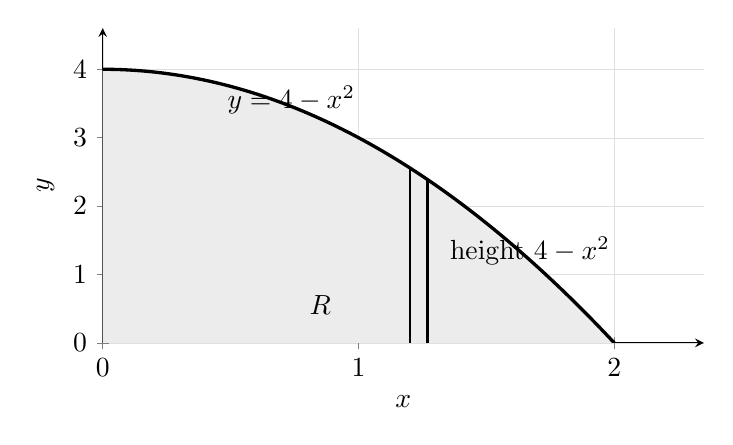
\begin{tikzpicture}
\begin{axis}[
    width=0.76\textwidth,
    height=0.46\textwidth,
    xmin=0, xmax=2.35,
    ymin=0, ymax=4.6,
    axis lines=left,
    xlabel={\(x\)},
    ylabel={\(y\)},
    xtick={0,1,2},
    ytick={0,1,2,3,4},
    grid=both,
    grid style={line width=.1pt, draw=gray!25},
]
\addplot[domain=0:2, samples=120, fill=gray!15, draw=none] {4-x^2} \closedcycle;
\addplot[very thick, domain=0:2.1, samples=120] {4-x^2};

% vertical strip
\draw[thick] (axis cs:1.2,0) -- (axis cs:1.2,2.56);
\draw[thick] (axis cs:1.27,0) -- (axis cs:1.27,2.39);
\node[anchor=west] at (axis cs:1.32,1.35) {height \(4-x^2\)};

\node[anchor=west] at (axis cs:0.45,3.55) {\(y=4-x^2\)};
\node at (axis cs:0.85,0.55) {\(R\)};
\end{axis}
\end{tikzpicture}
\caption{The same region can produce different integrals depending on what quantity is being measured.}
\label{fig:one-region-several-questions}
\end{figure}

\paragraph{Area.}
A vertical strip has height

\[
4-x^2
\]

and width \(dx\).  So

\[
A=\int_0^2 (4-x^2)\,dx.
\]

Compute:

\[
A=\left(4x-\frac{x^3}{3}\right)\Big|_0^2
=
8-\frac83
=
\boxed{\frac{16}{3}}.
\]

\paragraph{Volume around the \(x\)-axis.}
Rotating the region around the \(x\)-axis gives disk slices.  The radius is

\[
4-x^2.
\]

So

\[
V_x=\pi\int_0^2 (4-x^2)^2\,dx.
\]

Compute:

\[
V_x
=
\pi\int_0^2 (16-8x^2+x^4)\,dx.
\]

Thus

\[
V_x
=
\pi\left(16x-\frac{8x^3}{3}+\frac{x^5}{5}\right)\Big|_0^2.
\]

So

\[
V_x
=
\pi\left(32-\frac{64}{3}+\frac{32}{5}\right)
=
\boxed{\frac{256\pi}{15}}.
\]

\paragraph{Volume around the \(y\)-axis.}
Rotating the same region around the \(y\)-axis suggests shells.  A vertical strip has
radius \(x\), height \(4-x^2\), and thickness \(dx\).  Therefore

\[
V_y=2\pi\int_0^2 x(4-x^2)\,dx.
\]

Compute:

\[
V_y
=
2\pi\left(2x^2-\frac{x^4}{4}\right)\Big|_0^2
=
2\pi(8-4)
=
\boxed{8\pi}.
\]

\paragraph{Mass with varying density.}
Suppose \(R\) is a thin plate whose areal density depends only on \(x\):

\[
\sigma(x)=1+x.
\]

A vertical slice has area approximately

\[
(4-x^2)\,dx.
\]

So its mass is

\[
dm=(1+x)(4-x^2)\,dx.
\]

The total mass is

\[
m=\int_0^2 (1+x)(4-x^2)\,dx.
\]

Compute:

\[
m=\int_0^2 (4+4x-x^2-x^3)\,dx.
\]

Thus

\[
m=
\left(4x+2x^2-\frac{x^3}{3}-\frac{x^4}{4}\right)\Big|_0^2
=
8+8-\frac83-4
=
\boxed{\frac{28}{3}}.
\]

\paragraph{Average height.}
The average value of the top curve on \([0,2]\) is

\[
(4-x^2)_{\text{avg}}
=
\frac1{2-0}\int_0^2(4-x^2)\,dx.
\]

Since the area integral is \(16/3\),

\[
(4-x^2)_{\text{avg}}
=
\frac12\cdot\frac{16}{3}
=
\boxed{\frac83}.
\]

The region did not change.  The question changed.  That changed the small piece.

\[
\boxed{
\text{Same picture, different quantity, different integral.}
}
\]

\subsection{Concept checks}
\label{subsec:chapter10-concept-checks}

\begin{enumerate}
\item Why is area between curves computed as

\[
\int(\text{top}-\text{bottom})\,dx
\]

rather than

\[
\int(\text{bottom}-\text{top})\,dx?
\]

\item In the washer method, why is the washer area

\[
\pi R^2-\pi r^2
\]

and not

\[
\pi(R-r)^2?
\]

\item When rotating a region around the \(y\)-axis, why do vertical slices make shells
instead of washers?

\item Why does hydrostatic force on a vertical plate usually use horizontal strips?

\item What is the difference between density and total mass?

\item Why can a probability density be greater than \(1\) even though probabilities
cannot be greater than \(1\)?

\item What does the expected value of a probability density have in common with the
center of mass of a rod?

\item Why is arc length not usually

\[
\int_a^b |f'(x)|\,dx?
\]

\item What does the factor

\[
\sqrt{1+\bigl(f'(x)\bigr)^2}
\]

measure in the arc length formula?

\item In surface area of revolution, why does the formula contain a circumference factor?
\end{enumerate}

\subsection{Practice: set up the integral}
\label{subsec:chapter10-practice-setups}

For each problem, write the small piece first.  Then set up the integral.  Evaluate only
when the problem asks you to evaluate.

\begin{enumerate}
\item Find the area between

\[
y=\sqrt{x}
\qquad\text{and}\qquad
y=x^2
\]

on \([0,1]\).

\item Find the area enclosed by

\[
x=y^2
\qquad\text{and}\qquad
x=4-y^2.
\]

Use horizontal strips.

\item The region under

\[
y=\sqrt{x}
\]

from \(x=0\) to \(x=4\) is rotated around the \(x\)-axis.  Set up the disk-method
integral for the volume.

\item The same region is rotated around the \(y\)-axis.  Set up the shell-method integral
for the volume.

\item A solid has base bounded by

\[
y=x
\qquad\text{and}\qquad
y=x^2
\]

for \(0\le x\le1\).  Cross sections perpendicular to the \(x\)-axis are squares.  Set up
the volume integral.

\item A rod lies on \([0,3]\) and has linear density

\[
\lambda(x)=5+2x.
\]

Find its mass and set up the integral for its center of mass.

\item A spring has spring constant \(300\) N/m.  Find the work required to stretch it from
\(0.10\) m to \(0.40\) m beyond its natural length.

\item A rectangular tank is \(5\) ft long, \(3\) ft wide, and \(4\) ft deep.  It is full of water.
Set up the work integral needed to pump the water over the top edge.

\item A vertical triangular plate has vertex at the water surface and base \(6\) ft long at
depth \(4\) ft.  Set up the hydrostatic force integral on one side of the plate.

\item Let

\[
p(x)=cx^2,
\qquad 0\le x\le2.
\]

Find \(c\) so that \(p\) is a probability density.  Then set up the expected value
integral.

\item Set up and evaluate the arc length of

\[
y=\frac23x^{3/2}
\]

from \(x=0\) to \(x=3\).

\item Set up the surface area integral for rotating

\[
y=x^2,
\qquad 0\le x\le1,
\]

around the \(y\)-axis.
\end{enumerate}

\subsection{Project: compare volume methods}
\label{subsec:project-compare-volume-methods}

One solid can often be measured in more than one way.  The answer must be the same,
but the setup can look very different.

Let \(R\) be the region bounded by

\[
y=x
\]

and

\[
y=x^2
\]

for

\[
0\le x\le1.
\]

\paragraph{Part A: rotate around the \(y\)-axis.}

\begin{enumerate}
\item Sketch the region \(R\).

\item Use vertical shells.  A vertical strip has radius \(x\) and height \(x-x^2\).  Show that

\[
V=2\pi\int_0^1 x(x-x^2)\,dx.
\]

Evaluate the integral.

\item Use horizontal washers.  Rewrite the boundaries as

\[
x=y
\qquad\text{and}\qquad
x=\sqrt y.
\]

For \(0\le y\le1\), identify the outer and inner radii.  Show that

\[
V=\pi\int_0^1 (y-y^2)\,dy.
\]

Evaluate the integral.

\item Verify that both methods give

\[
\boxed{\frac{\pi}{6}}.
\]
\end{enumerate}

\paragraph{Part B: rotate around the \(x\)-axis.}

\begin{enumerate}
\item Use vertical washers.  Show that

\[
V=\pi\int_0^1 (x^2-x^4)\,dx.
\]

\item Use horizontal shells.  A horizontal strip has radius \(y\) and length

\[
\sqrt y-y.
\]

Show that

\[
V=2\pi\int_0^1 y(\sqrt y-y)\,dy.
\]

\item Verify that both methods give

\[
\boxed{\frac{2\pi}{15}}.
\]
\end{enumerate}

\paragraph{Part C: compare the methods.}

Write a short explanation answering these questions.

\begin{enumerate}
\item Which method was simpler for rotation around the \(y\)-axis?
\item Which method was simpler for rotation around the \(x\)-axis?
\item What made one method simpler than the other: fewer integrals, easier bounds, or a
simpler integrand?
\item Why is it useful to know more than one method?
\end{enumerate}

\begin{quote}
\textbf{What the project tests.}
The disk, washer, and shell methods are not separate tricks.  They are different ways of
choosing the small piece.  A good method is the one that makes the small piece easy to
describe.
\end{quote}

\subsection{Project: work needed to pump out a real tank shape}
\label{subsec:project-pump-real-tank-shape}

Exact formulas are useful, but real tanks are not always cones, cylinders, or rectangular
boxes.  Sometimes the most honest description is measured data.

A closed cistern is \(8\) feet tall.  Water is pumped out through a small opening at the top,
which is at height \(8\) feet above the bottom.  The following table gives measured
horizontal cross-sectional areas of the water region at different heights.

\begin{center}
\begin{tabular}{c|ccccccccc}
\(y\) (ft above bottom) & \(0\) & \(1\) & \(2\) & \(3\) & \(4\) & \(5\) & \(6\) & \(7\) & \(8\) \\ \hline
\(A(y)\) (ft\(^2\)) & \(0\) & \(18\) & \(31\) & \(40\) & \(44\) & \(40\) & \(31\) & \(18\) & \(0\)
\end{tabular}
\end{center}

Assume the cistern is full of water.  Use

\[
\gamma=62.4\text{ lb/ft}^3
\]

for the weight density of water.

A thin layer at height \(y\) has volume approximately

\[
A(y)\,dy.
\]

Its weight is

\[
62.4A(y)\,dy.
\]

It must be lifted distance

\[
8-y.
\]

So the work is

\[
\boxed{
W=62.4\int_0^8 A(y)(8-y)\,dy.
}
\]

Because \(A(y)\) is known only from data, estimate the integral.

\paragraph{A trapezoid estimate.}
Let

\[
B(y)=A(y)(8-y).
\]

Then

\[
W=62.4\int_0^8 B(y)\,dy.
\]

The table for \(B(y)\) is:

\begin{center}
\begin{tabular}{c|ccccccccc}
\(y\) & \(0\) & \(1\) & \(2\) & \(3\) & \(4\) & \(5\) & \(6\) & \(7\) & \(8\) \\ \hline
\(B(y)\) & \(0\) & \(126\) & \(186\) & \(200\) & \(176\) & \(120\) & \(62\) & \(18\) & \(0\)
\end{tabular}
\end{center}

Using trapezoids with \(\Delta y=1\),

\[
\int_0^8 B(y)\,dy
\approx
\frac12B(0)+B(1)+B(2)+\cdots+B(7)+\frac12B(8).
\]

So

\[
\int_0^8 B(y)\,dy
\approx
126+186+200+176+120+62+18
=
888.
\]

Therefore

\[
W\approx 62.4(888)=\boxed{55{,}411.2}
\]

foot-pounds.

\paragraph{Questions for the project.}

\begin{enumerate}
\item Why should we apply the trapezoid rule to

\[
B(y)=A(y)(8-y)
\]

rather than to \(A(y)\) alone?

\item Which layers contribute most to the work?  Is it always the layer with the largest
area?

\item If the water must be pumped to a spout \(1\) foot above the top of the cistern, how
does the formula change?

\item Suppose measurements are expensive and you can add only two more height
measurements.  Where would you place them?  Explain your choice.

\item Estimate the work again using any reasonable improved method, and compare your
answer with \(55{,}411.2\) foot-pounds.
\end{enumerate}

\begin{quote}
\textbf{What the project tests.}
The integral model comes from the small piece

\[
dW=(\text{weight of layer})(\text{lifting distance}).
\]

The data only change how we estimate the integral.
\end{quote}

\subsection{Where this points}
\label{subsec:chapter10-hook-techniques-of-integration}

This chapter has shown why integrals matter.

They measure area, volume, mass, center of mass, work, hydrostatic force, average
value, probability, arc length, and surface area.

But setting up an integral is not the same as evaluating it.

Even simple applications can produce integrals such as

\[
\int x e^x\,dx,
\qquad
\int \sin^5 x\cos^2 x\,dx,
\qquad
\int \sqrt{9-x^2}\,dx,
\qquad
\int \frac{x^2+1}{x^3-x}\,dx.
\]

Substitution will not handle all of these.  Some require reversing the product rule.
Some require trigonometric identities.  Some require a clever triangle.  Some require
partial fractions.  Some have no elementary antiderivative at all.

That is the next problem.

\[
\boxed{
\text{The small piece tells us what to integrate.  Now we need better ways to integrate it.}
}
\]

The next chapter develops techniques for finding antiderivatives when substitution alone
is not enough.
